\documentclass[1p]{elsarticle_modified}
%\bibliographystyle{elsarticle-num}

%\usepackage[colorlinks]{hyperref}
%\usepackage{abbrmath_seonhwa} %\Abb, \Ascr, \Acal ,\Abf, \Afrak
\usepackage{amsfonts}
\usepackage{amssymb}
\usepackage{amsmath}
\usepackage{amsthm}
\usepackage{scalefnt}
\usepackage{amsbsy}
\usepackage{kotex}
\usepackage{caption}
\usepackage{subfig}
\usepackage{color}
\usepackage{graphicx}
\usepackage{xcolor} %% white, black, red, green, blue, cyan, magenta, yellow
\usepackage{float}
\usepackage{setspace}
\usepackage{hyperref}

\usepackage{tikz}
\usetikzlibrary{arrows}

\usepackage{multirow}
\usepackage{array} % fixed length table
\usepackage{hhline}

%%%%%%%%%%%%%%%%%%%%%
\makeatletter
\renewcommand*\env@matrix[1][\arraystretch]{%
	\edef\arraystretch{#1}%
	\hskip -\arraycolsep
	\let\@ifnextchar\new@ifnextchar
	\array{*\c@MaxMatrixCols c}}
\makeatother %https://tex.stackexchange.com/questions/14071/how-can-i-increase-the-line-spacing-in-a-matrix
%%%%%%%%%%%%%%%

\usepackage[normalem]{ulem}

\newcommand{\msout}[1]{\ifmmode\text{\sout{\ensuremath{#1}}}\else\sout{#1}\fi}
%SOURCE: \msout is \stkout macro in https://tex.stackexchange.com/questions/20609/strikeout-in-math-mode

\newcommand{\cancel}[1]{
	\ifmmode
	{\color{red}\msout{#1}}
	\else
	{\color{red}\sout{#1}}
	\fi
}

\newcommand{\add}[1]{
	{\color{blue}\uwave{#1}}
}

\newcommand{\replace}[2]{
	\ifmmode
	{\color{red}\msout{#1}}{\color{blue}\uwave{#2}}
	\else
	{\color{red}\sout{#1}}{\color{blue}\uwave{#2}}
	\fi
}

\newcommand{\Sol}{\mathcal{S}} %segment
\newcommand{\D}{D} %diagram
\newcommand{\A}{\mathcal{A}} %arc


%%%%%%%%%%%%%%%%%%%%%%%%%%%%%5 test

\def\sl{\operatorname{\textup{SL}}(2,\Cbb)}
\def\psl{\operatorname{\textup{PSL}}(2,\Cbb)}
\def\quan{\mkern 1mu \triangleright \mkern 1mu}

\theoremstyle{definition}
\newtheorem{thm}{Theorem}[section]
\newtheorem{prop}[thm]{Proposition}
\newtheorem{lem}[thm]{Lemma}
\newtheorem{ques}[thm]{Question}
\newtheorem{cor}[thm]{Corollary}
\newtheorem{defn}[thm]{Definition}
\newtheorem{exam}[thm]{Example}
\newtheorem{rmk}[thm]{Remark}
\newtheorem{alg}[thm]{Algorithm}

\newcommand{\I}{\sqrt{-1}}
\begin{document}

%\begin{frontmatter}
%
%\title{Boundary parabolic representations of knots up to 8 crossings}
%
%%% Group authors per affiliation:
%\author{Yunhi Cho} 
%\address{Department of Mathematics, University of Seoul, Seoul, Korea}
%\ead{yhcho@uos.ac.kr}
%
%
%\author{Seonhwa Kim} %\fnref{s_kim}}
%\address{Center for Geometry and Physics, Institute for Basic Science, Pohang, 37673, Korea}
%\ead{ryeona17@ibs.re.kr}
%
%\author{Hyuk Kim}
%\address{Department of Mathematical Sciences, Seoul National University, Seoul 08826, Korea}
%\ead{hyukkim@snu.ac.kr}
%
%\author{Seokbeom Yoon}
%\address{Department of Mathematical Sciences, Seoul National University, Seoul, 08826,  Korea}
%\ead{sbyoon15@snu.ac.kr}
%
%\begin{abstract}
%We find all boundary parabolic representation of knots up to 8 crossings.
%
%\end{abstract}
%\begin{keyword}
%    \MSC[2010] 57M25 
%\end{keyword}
%
%\end{frontmatter}

%\linenumbers
%\tableofcontents
%
\newcommand\colored[1]{\textcolor{white}{\rule[-0.35ex]{0.8em}{1.4ex}}\kern-0.8em\color{red} #1}%
%\newcommand\colored[1]{\textcolor{white}{ #1}\kern-2.17ex	\textcolor{white}{ #1}\kern-1.81ex	\textcolor{white}{ #1}\kern-2.15ex\color{red}#1	}

{\Large $\underline{12a_{0486}~(K12a_{0486})}$}

\setlength{\tabcolsep}{10pt}
\renewcommand{\arraystretch}{1.6}
\vspace{1cm}\begin{tabular}{m{100pt}>{\centering\arraybackslash}m{274pt}}
\multirow{5}{120pt}{
	\centering
	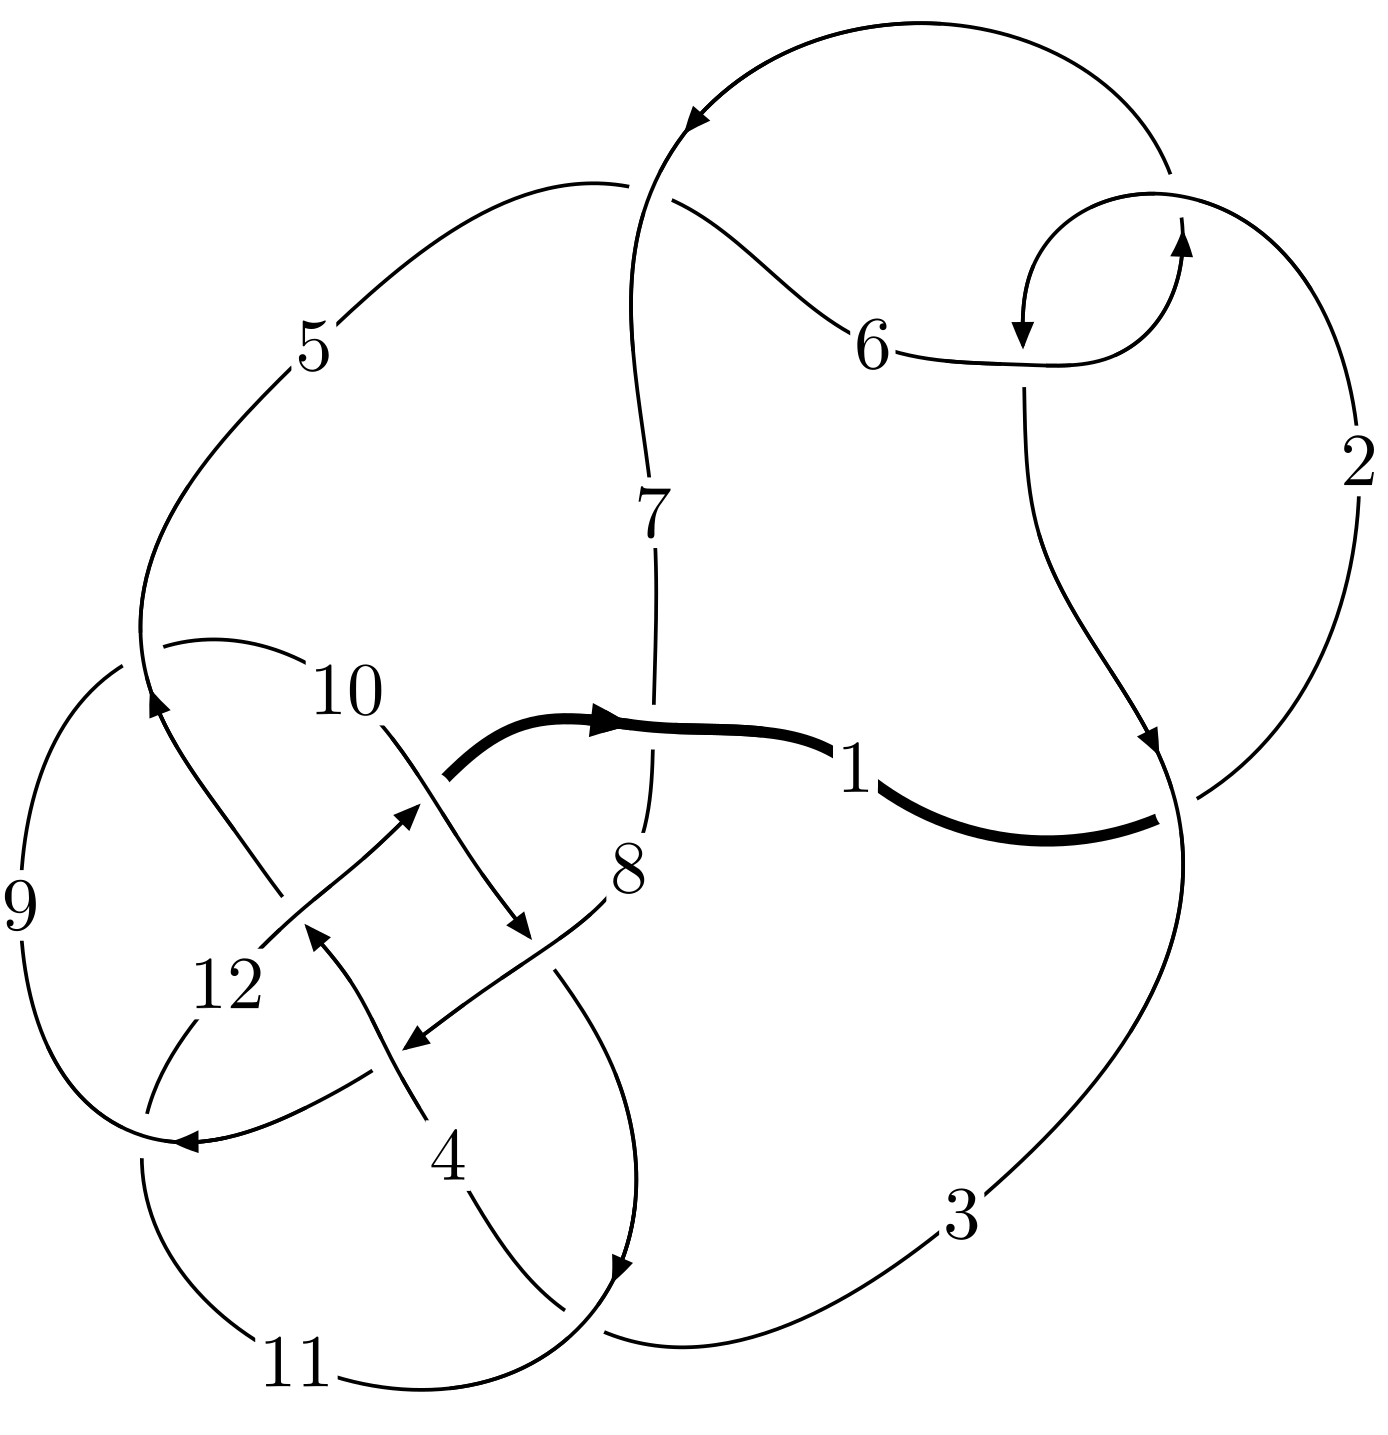
\includegraphics[width=112pt]{../../../GIT/diagram.site/Diagrams/png/1287_12a_0486.png}\\
\ \ \ A knot diagram\footnotemark}&
\allowdisplaybreaks
\textbf{Linearized knot diagam} \\
\cline{2-2}
 &
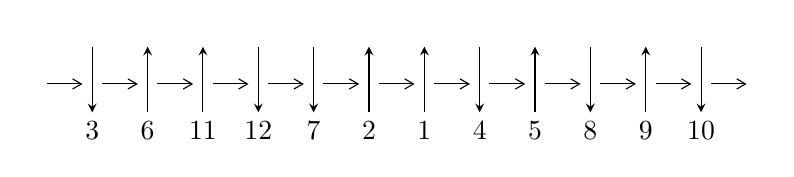
\begin{tikzpicture}[x=20pt, y=17pt]
	% nodes
	\node (C0) at (0, 0) {};
	\node (C1) at (1, 0) {};
	\node (C1U) at (1, +1) {};
	\node (C1D) at (1, -1) {3};

	\node (C2) at (2, 0) {};
	\node (C2U) at (2, +1) {};
	\node (C2D) at (2, -1) {6};

	\node (C3) at (3, 0) {};
	\node (C3U) at (3, +1) {};
	\node (C3D) at (3, -1) {11};

	\node (C4) at (4, 0) {};
	\node (C4U) at (4, +1) {};
	\node (C4D) at (4, -1) {12};

	\node (C5) at (5, 0) {};
	\node (C5U) at (5, +1) {};
	\node (C5D) at (5, -1) {7};

	\node (C6) at (6, 0) {};
	\node (C6U) at (6, +1) {};
	\node (C6D) at (6, -1) {2};

	\node (C7) at (7, 0) {};
	\node (C7U) at (7, +1) {};
	\node (C7D) at (7, -1) {1};

	\node (C8) at (8, 0) {};
	\node (C8U) at (8, +1) {};
	\node (C8D) at (8, -1) {4};

	\node (C9) at (9, 0) {};
	\node (C9U) at (9, +1) {};
	\node (C9D) at (9, -1) {5};

	\node (C10) at (10, 0) {};
	\node (C10U) at (10, +1) {};
	\node (C10D) at (10, -1) {8};

	\node (C11) at (11, 0) {};
	\node (C11U) at (11, +1) {};
	\node (C11D) at (11, -1) {9};

	\node (C12) at (12, 0) {};
	\node (C12U) at (12, +1) {};
	\node (C12D) at (12, -1) {10};
	\node (C13) at (13, 0) {};

	% arrows
	\draw[->,>={angle 60}]
	(C0) edge (C1) (C1) edge (C2) (C2) edge (C3) (C3) edge (C4) (C4) edge (C5) (C5) edge (C6) (C6) edge (C7) (C7) edge (C8) (C8) edge (C9) (C9) edge (C10) (C10) edge (C11) (C11) edge (C12) (C12) edge (C13) ;	\draw[->,>=stealth]
	(C1U) edge (C1D) (C2D) edge (C2U) (C3D) edge (C3U) (C4U) edge (C4D) (C5U) edge (C5D) (C6D) edge (C6U) (C7D) edge (C7U) (C8U) edge (C8D) (C9D) edge (C9U) (C10U) edge (C10D) (C11D) edge (C11U) (C12U) edge (C12D) ;
	\end{tikzpicture} \\
\hhline{~~} \\& 
\textbf{Solving Sequence} \\ \cline{2-2} 
 &
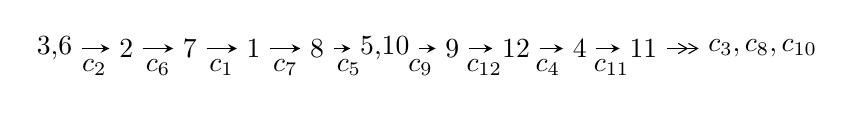
\begin{tikzpicture}[x=23pt, y=7pt]
	% node
	\node (A0) at (-1/8, 0) {3,6};
	\node (A1) at (1, 0) {2};
	\node (A2) at (2, 0) {7};
	\node (A3) at (3, 0) {1};
	\node (A4) at (4, 0) {8};
	\node (A5) at (81/16, 0) {5,10};
	\node (A6) at (49/8, 0) {9};
	\node (A7) at (57/8, 0) {12};
	\node (A8) at (65/8, 0) {4};
	\node (A9) at (73/8, 0) {11};
	\node (C1) at (1/2, -1) {$c_{2}$};
	\node (C2) at (3/2, -1) {$c_{6}$};
	\node (C3) at (5/2, -1) {$c_{1}$};
	\node (C4) at (7/2, -1) {$c_{7}$};
	\node (C5) at (9/2, -1) {$c_{5}$};
	\node (C6) at (45/8, -1) {$c_{9}$};
	\node (C7) at (53/8, -1) {$c_{12}$};
	\node (C8) at (61/8, -1) {$c_{4}$};
	\node (C9) at (69/8, -1) {$c_{11}$};
	\node (A10) at (11, 0) {$c_{3},c_{8},c_{10}$};

	% edge
	\draw[->,>=stealth]	
	(A0) edge (A1) (A1) edge (A2) (A2) edge (A3) (A3) edge (A4) (A4) edge (A5) (A5) edge (A6) (A6) edge (A7) (A7) edge (A8) (A8) edge (A9) ;
	\draw[->>,>={angle 60}]	
	(A9) edge (A10);
\end{tikzpicture} \\ 

\end{tabular} \\

\footnotetext{
The image of knot diagram is generated by the software ``\textbf{Draw programme}" developed by Andrew Bartholomew(\url{http://www.layer8.co.uk/maths/draw/index.htm\#Running-draw}), where we modified some parts for our purpose(\url{https://github.com/CATsTAILs/LinksPainter}).
}\phantom \\ \newline 
\centering \textbf{Ideals for irreducible components\footnotemark of $X_{\text{par}}$} 
 
\begin{align*}
I^u_{1}&=\langle 
-48599558 u^{68}-169298104 u^{67}+\cdots+17100943 b-315531735,\\
\phantom{I^u_{1}}&\phantom{= \langle  }350511433 u^{68}+1020261118 u^{67}+\cdots+119706601 a-2664075662,\;u^{69}+5 u^{68}+\cdots-11 u+7\rangle \\
I^u_{2}&=\langle 
-352821 u^{46} a-5119679 u^{46}+\cdots-1763091 a+4390751,\;- u^{46} a-4 u^{46}+\cdots+4 a-2,\\
\phantom{I^u_{2}}&\phantom{= \langle  }u^{47}-2 u^{46}+\cdots-2 u+1\rangle \\
I^u_{3}&=\langle 
u^{22}+u^{21}+\cdots+b+3 u,\;u^{23}-2 u^{22}+\cdots+a+3,\;u^{24}-2 u^{23}+\cdots+7 u^2+1\rangle \\
I^u_{4}&=\langle 
a u+b+u+1,\;a^2-3 a u-3 u-2,\;u^2+u+1\rangle \\
\\
I^v_{1}&=\langle 
a,\;b+1,\;v-1\rangle \\
\end{align*}
\raggedright * 5 irreducible components of $\dim_{\mathbb{C}}=0$, with total 192 representations.\\
\footnotetext{All coefficients of polynomials are rational numbers. But the coefficients are sometimes approximated in decimal forms when there is not enough margin.}
\newpage
\renewcommand{\arraystretch}{1}
\centering \section*{I. $I^u_{1}= \langle -4.86\times10^{7} u^{68}-1.69\times10^{8} u^{67}+\cdots+1.71\times10^{7} b-3.16\times10^{8},\;3.51\times10^{8} u^{68}+1.02\times10^{9} u^{67}+\cdots+1.20\times10^{8} a-2.66\times10^{9},\;u^{69}+5 u^{68}+\cdots-11 u+7 \rangle$}
\flushleft \textbf{(i) Arc colorings}\\
\begin{tabular}{m{7pt} m{180pt} m{7pt} m{180pt} }
\flushright $a_{3}=$&$\begin{pmatrix}1\\0\end{pmatrix}$ \\
\flushright $a_{6}=$&$\begin{pmatrix}0\\u\end{pmatrix}$ \\
\flushright $a_{2}=$&$\begin{pmatrix}1\\u^2\end{pmatrix}$ \\
\flushright $a_{7}=$&$\begin{pmatrix}u\\u^3+u\end{pmatrix}$ \\
\flushright $a_{1}=$&$\begin{pmatrix}u^2+1\\u^2\end{pmatrix}$ \\
\flushright $a_{8}=$&$\begin{pmatrix}u^7+2 u^5+2 u^3+2 u\\u^7+u^5+2 u^3+u\end{pmatrix}$ \\
\flushright $a_{5}=$&$\begin{pmatrix}u^3\\u^5+u^3+u\end{pmatrix}$ \\
\flushright $a_{10}=$&$\begin{pmatrix}-2.92809 u^{68}-8.52301 u^{67}+\cdots-75.4142 u+22.2550\\2.84192 u^{68}+9.89993 u^{67}+\cdots-49.7328 u+18.4511\end{pmatrix}$ \\
\flushright $a_{9}=$&$\begin{pmatrix}-4.76650 u^{68}-13.2256 u^{67}+\cdots-105.769 u+29.5256\\-1.57547 u^{68}-5.78395 u^{67}+\cdots-56.6428 u+13.2040\end{pmatrix}$ \\
\flushright $a_{12}=$&$\begin{pmatrix}-4.76183 u^{68}-9.61536 u^{67}+\cdots-111.548 u+35.3483\\-3.57547 u^{68}-12.7839 u^{67}+\cdots-42.6428 u+6.20396\end{pmatrix}$ \\
\flushright $a_{4}=$&$\begin{pmatrix}-2.98023 u^{68}-12.1415 u^{67}+\cdots+22.7597 u-10.5704\\-2.77581 u^{68}-13.7928 u^{67}+\cdots+33.0385 u-16.8236\end{pmatrix}$ \\
\flushright $a_{11}=$&$\begin{pmatrix}8.01122 u^{68}+28.2908 u^{67}+\cdots+64.2914 u-4.00348\\2.70124 u^{68}+10.8019 u^{67}+\cdots-12.4433 u+9.09453\end{pmatrix}$\\&\end{tabular}
\flushleft \textbf{(ii) Obstruction class $= -1$}\\~\\
\flushleft \textbf{(iii) Cusp Shapes $= -\frac{53809100}{17100943} u^{68}-\frac{239622692}{17100943} u^{67}+\cdots+\frac{686921128}{17100943} u-\frac{253153132}{17100943}$}\\~\\
\newpage\renewcommand{\arraystretch}{1}
\flushleft \textbf{(iv) u-Polynomials at the component}\newline \\
\begin{tabular}{m{50pt}|m{274pt}}
Crossings & \hspace{64pt}u-Polynomials at each crossing \\
\hline $$\begin{aligned}c_{1},c_{5}\end{aligned}$$&$\begin{aligned}
&u^{69}+23 u^{68}+\cdots+65 u-49
\end{aligned}$\\
\hline $$\begin{aligned}c_{2},c_{6}\end{aligned}$$&$\begin{aligned}
&u^{69}-5 u^{68}+\cdots-11 u-7
\end{aligned}$\\
\hline $$\begin{aligned}c_{3},c_{9}\end{aligned}$$&$\begin{aligned}
&u^{69}-2 u^{68}+\cdots-3 u-1
\end{aligned}$\\
\hline $$\begin{aligned}c_{4},c_{8}\end{aligned}$$&$\begin{aligned}
&u^{69}- u^{68}+\cdots-2 u-1
\end{aligned}$\\
\hline $$\begin{aligned}c_{7}\end{aligned}$$&$\begin{aligned}
&u^{69}+25 u^{68}+\cdots-59915 u-3703
\end{aligned}$\\
\hline $$\begin{aligned}c_{10},c_{12}\end{aligned}$$&$\begin{aligned}
&u^{69}+10 u^{68}+\cdots+29 u-1
\end{aligned}$\\
\hline $$\begin{aligned}c_{11}\end{aligned}$$&$\begin{aligned}
&u^{69}+38 u^{68}+\cdots-64 u-7
\end{aligned}$\\
\hline
\end{tabular}\\~\\
\newpage\renewcommand{\arraystretch}{1}
\flushleft \textbf{(v) Riley Polynomials at the component}\newline \\
\begin{tabular}{m{50pt}|m{274pt}}
Crossings & \hspace{64pt}Riley Polynomials at each crossing \\
\hline $$\begin{aligned}c_{1},c_{5}\end{aligned}$$&$\begin{aligned}
&y^{69}+51 y^{68}+\cdots+29901 y-2401
\end{aligned}$\\
\hline $$\begin{aligned}c_{2},c_{6}\end{aligned}$$&$\begin{aligned}
&y^{69}+23 y^{68}+\cdots+65 y-49
\end{aligned}$\\
\hline $$\begin{aligned}c_{3},c_{9}\end{aligned}$$&$\begin{aligned}
&y^{69}-6 y^{68}+\cdots-33 y-1
\end{aligned}$\\
\hline $$\begin{aligned}c_{4},c_{8}\end{aligned}$$&$\begin{aligned}
&y^{69}-29 y^{68}+\cdots+76 y-1
\end{aligned}$\\
\hline $$\begin{aligned}c_{7}\end{aligned}$$&$\begin{aligned}
&y^{69}+3 y^{68}+\cdots-816311009 y-13712209
\end{aligned}$\\
\hline $$\begin{aligned}c_{10},c_{12}\end{aligned}$$&$\begin{aligned}
&y^{69}-42 y^{68}+\cdots+27 y-1
\end{aligned}$\\
\hline $$\begin{aligned}c_{11}\end{aligned}$$&$\begin{aligned}
&y^{69}+50 y^{67}+\cdots+134 y-49
\end{aligned}$\\
\hline
\end{tabular}\\~\\
\newpage\flushleft \textbf{(vi) Complex Volumes and Cusp Shapes}
$$\begin{array}{c|c|c}  
\text{Solutions to }I^u_{1}& \I (\text{vol} + \sqrt{-1}CS) & \text{Cusp shape}\\
 \hline 
\begin{aligned}
u &= -0.012222 + 1.002130 I \\
a &= -1.121370 + 0.553514 I \\
b &= \phantom{-}1.66113 + 0.68765 I\end{aligned}
 & -5.00379 - 0.12361 I & -9.98584 + 0. I\phantom{ +0.000000I} \\ \hline\begin{aligned}
u &= -0.012222 - 1.002130 I \\
a &= -1.121370 - 0.553514 I \\
b &= \phantom{-}1.66113 - 0.68765 I\end{aligned}
 & -5.00379 + 0.12361 I & -9.98584 + 0. I\phantom{ +0.000000I} \\ \hline\begin{aligned}
u &= \phantom{-}0.716065 + 0.706433 I \\
a &= -1.78731 - 1.65142 I \\
b &= -0.623796 - 0.900743 I\end{aligned}
 & \phantom{-}0.0540759 - 0.0939258 I & \phantom{-0.000000 } 0 \\ \hline\begin{aligned}
u &= \phantom{-}0.716065 - 0.706433 I \\
a &= -1.78731 + 1.65142 I \\
b &= -0.623796 + 0.900743 I\end{aligned}
 & \phantom{-}0.0540759 + 0.0939258 I & \phantom{-0.000000 } 0 \\ \hline\begin{aligned}
u &= -0.683285 + 0.702977 I \\
a &= -1.68834 - 0.68669 I \\
b &= -1.82191 + 0.42380 I\end{aligned}
 & -0.234320 - 0.001152 I & -2.25563 + 0. I\phantom{ +0.000000I} \\ \hline\begin{aligned}
u &= -0.683285 - 0.702977 I \\
a &= -1.68834 + 0.68669 I \\
b &= -1.82191 - 0.42380 I\end{aligned}
 & -0.234320 + 0.001152 I & -2.25563 + 0. I\phantom{ +0.000000I} \\ \hline\begin{aligned}
u &= -0.793801 + 0.571976 I \\
a &= \phantom{-}1.148810 + 0.200493 I \\
b &= \phantom{-}0.957086 - 0.158430 I\end{aligned}
 & -0.92159 - 2.20912 I & -4.61148 + 3.51139 I \\ \hline\begin{aligned}
u &= -0.793801 - 0.571976 I \\
a &= \phantom{-}1.148810 - 0.200493 I \\
b &= \phantom{-}0.957086 + 0.158430 I\end{aligned}
 & -0.92159 + 2.20912 I & -4.61148 - 3.51139 I \\ \hline\begin{aligned}
u &= \phantom{-}0.141687 + 1.029870 I \\
a &= -0.843291 - 0.549722 I \\
b &= \phantom{-}1.237290 + 0.564726 I\end{aligned}
 & -5.58220 + 1.94498 I & -10.57738 + 0. I\phantom{ +0.000000I} \\ \hline\begin{aligned}
u &= \phantom{-}0.141687 - 1.029870 I \\
a &= -0.843291 + 0.549722 I \\
b &= \phantom{-}1.237290 - 0.564726 I\end{aligned}
 & -5.58220 - 1.94498 I & -10.57738 + 0. I\phantom{ +0.000000I}\\
 \hline 
 \end{array}$$\newpage$$\begin{array}{c|c|c}  
\text{Solutions to }I^u_{1}& \I (\text{vol} + \sqrt{-1}CS) & \text{Cusp shape}\\
 \hline 
\begin{aligned}
u &= -0.796333 + 0.677780 I \\
a &= -2.41597 + 0.72004 I \\
b &= -2.10792 + 1.43766 I\end{aligned}
 & \phantom{-}0.15968 + 5.61109 I & \phantom{-0.000000 } 0 \\ \hline\begin{aligned}
u &= -0.796333 - 0.677780 I \\
a &= -2.41597 - 0.72004 I \\
b &= -2.10792 - 1.43766 I\end{aligned}
 & \phantom{-}0.15968 - 5.61109 I & \phantom{-0.000000 } 0 \\ \hline\begin{aligned}
u &= \phantom{-}0.110513 + 1.048830 I \\
a &= -1.236350 + 0.224439 I \\
b &= \phantom{-}2.06677 - 0.35387 I\end{aligned}
 & -6.03215 + 5.53076 I & \phantom{-0.000000 } 0 \\ \hline\begin{aligned}
u &= \phantom{-}0.110513 - 1.048830 I \\
a &= -1.236350 - 0.224439 I \\
b &= \phantom{-}2.06677 + 0.35387 I\end{aligned}
 & -6.03215 - 5.53076 I & \phantom{-0.000000 } 0 \\ \hline\begin{aligned}
u &= -0.119600 + 0.926304 I \\
a &= \phantom{-}0.219849 - 0.770724 I \\
b &= -0.850774 - 0.031966 I\end{aligned}
 & -1.43506 - 1.95242 I & -2.33460 + 4.04464 I \\ \hline\begin{aligned}
u &= -0.119600 - 0.926304 I \\
a &= \phantom{-}0.219849 + 0.770724 I \\
b &= -0.850774 + 0.031966 I\end{aligned}
 & -1.43506 + 1.95242 I & -2.33460 - 4.04464 I \\ \hline\begin{aligned}
u &= -0.837875 + 0.662257 I \\
a &= \phantom{-}2.29743 - 0.93819 I \\
b &= \phantom{-}1.91355 - 1.36492 I\end{aligned}
 & \phantom{-}1.6483 + 14.5043 I & \phantom{-0.000000 } 0 \\ \hline\begin{aligned}
u &= -0.837875 - 0.662257 I \\
a &= \phantom{-}2.29743 + 0.93819 I \\
b &= \phantom{-}1.91355 + 1.36492 I\end{aligned}
 & \phantom{-}1.6483 - 14.5043 I & \phantom{-0.000000 } 0 \\ \hline\begin{aligned}
u &= \phantom{-}0.777141 + 0.736280 I \\
a &= \phantom{-}1.149780 + 0.578014 I \\
b &= \phantom{-}0.491520 + 0.431357 I\end{aligned}
 & \phantom{-}4.40070 - 1.06842 I & \phantom{-0.000000 } 0 \\ \hline\begin{aligned}
u &= \phantom{-}0.777141 - 0.736280 I \\
a &= \phantom{-}1.149780 - 0.578014 I \\
b &= \phantom{-}0.491520 - 0.431357 I\end{aligned}
 & \phantom{-}4.40070 + 1.06842 I & \phantom{-0.000000 } 0\\
 \hline 
 \end{array}$$\newpage$$\begin{array}{c|c|c}  
\text{Solutions to }I^u_{1}& \I (\text{vol} + \sqrt{-1}CS) & \text{Cusp shape}\\
 \hline 
\begin{aligned}
u &= \phantom{-}0.541394 + 0.923763 I \\
a &= -1.36122 - 1.59201 I \\
b &= \phantom{-}0.267146 - 0.903066 I\end{aligned}
 & -3.42369 + 3.69120 I & \phantom{-0.000000 } 0 \\ \hline\begin{aligned}
u &= \phantom{-}0.541394 - 0.923763 I \\
a &= -1.36122 + 1.59201 I \\
b &= \phantom{-}0.267146 + 0.903066 I\end{aligned}
 & -3.42369 - 3.69120 I & \phantom{-0.000000 } 0 \\ \hline\begin{aligned}
u &= -0.819723 + 0.709991 I \\
a &= -1.252450 - 0.288105 I \\
b &= -1.385820 - 0.016383 I\end{aligned}
 & \phantom{-}0.87380 + 1.64675 I & \phantom{-0.000000 } 0 \\ \hline\begin{aligned}
u &= -0.819723 - 0.709991 I \\
a &= -1.252450 + 0.288105 I \\
b &= -1.385820 + 0.016383 I\end{aligned}
 & \phantom{-}0.87380 - 1.64675 I & \phantom{-0.000000 } 0 \\ \hline\begin{aligned}
u &= \phantom{-}0.554061 + 0.946702 I \\
a &= \phantom{-}0.09644 - 2.39009 I \\
b &= \phantom{-}1.003420 - 0.616051 I\end{aligned}
 & -3.54428 + 0.34170 I & \phantom{-0.000000 } 0 \\ \hline\begin{aligned}
u &= \phantom{-}0.554061 - 0.946702 I \\
a &= \phantom{-}0.09644 + 2.39009 I \\
b &= \phantom{-}1.003420 + 0.616051 I\end{aligned}
 & -3.54428 - 0.34170 I & \phantom{-0.000000 } 0 \\ \hline\begin{aligned}
u &= -0.745478 + 0.805661 I \\
a &= \phantom{-}0.757979 - 0.428250 I \\
b &= \phantom{-}0.54619 - 1.38301 I\end{aligned}
 & \phantom{-}2.31641 - 3.75915 I & \phantom{-0.000000 } 0 \\ \hline\begin{aligned}
u &= -0.745478 - 0.805661 I \\
a &= \phantom{-}0.757979 + 0.428250 I \\
b &= \phantom{-}0.54619 + 1.38301 I\end{aligned}
 & \phantom{-}2.31641 + 3.75915 I & \phantom{-0.000000 } 0 \\ \hline\begin{aligned}
u &= \phantom{-}0.139797 + 1.097740 I \\
a &= \phantom{-}0.958448 + 0.089891 I \\
b &= -2.02653 + 0.54635 I\end{aligned}
 & -5.0428 + 14.1417 I & \phantom{-0.000000 } 0 \\ \hline\begin{aligned}
u &= \phantom{-}0.139797 - 1.097740 I \\
a &= \phantom{-}0.958448 - 0.089891 I \\
b &= -2.02653 - 0.54635 I\end{aligned}
 & -5.0428 - 14.1417 I & \phantom{-0.000000 } 0\\
 \hline 
 \end{array}$$\newpage$$\begin{array}{c|c|c}  
\text{Solutions to }I^u_{1}& \I (\text{vol} + \sqrt{-1}CS) & \text{Cusp shape}\\
 \hline 
\begin{aligned}
u &= \phantom{-}0.063890 + 1.113210 I \\
a &= \phantom{-}0.404800 + 0.058459 I \\
b &= -1.167720 - 0.501445 I\end{aligned}
 & -6.98700 - 3.23243 I & \phantom{-0.000000 } 0 \\ \hline\begin{aligned}
u &= \phantom{-}0.063890 - 1.113210 I \\
a &= \phantom{-}0.404800 - 0.058459 I \\
b &= -1.167720 + 0.501445 I\end{aligned}
 & -6.98700 + 3.23243 I & \phantom{-0.000000 } 0 \\ \hline\begin{aligned}
u &= -0.448141 + 0.761288 I \\
a &= \phantom{-}0.546214 - 0.397562 I \\
b &= -0.055472 - 0.575637 I\end{aligned}
 & \phantom{-}0.01707 - 1.74830 I & -0.18091 + 2.95800 I \\ \hline\begin{aligned}
u &= -0.448141 - 0.761288 I \\
a &= \phantom{-}0.546214 + 0.397562 I \\
b &= -0.055472 + 0.575637 I\end{aligned}
 & \phantom{-}0.01707 + 1.74830 I & -0.18091 - 2.95800 I \\ \hline\begin{aligned}
u &= \phantom{-}0.485720 + 1.018670 I \\
a &= -0.29913 + 1.96319 I \\
b &= -1.205210 + 0.213225 I\end{aligned}
 & -2.96219 - 7.43047 I & \phantom{-0.000000 } 0 \\ \hline\begin{aligned}
u &= \phantom{-}0.485720 - 1.018670 I \\
a &= -0.29913 - 1.96319 I \\
b &= -1.205210 - 0.213225 I\end{aligned}
 & -2.96219 + 7.43047 I & \phantom{-0.000000 } 0 \\ \hline\begin{aligned}
u &= -0.712951 + 0.920207 I \\
a &= \phantom{-}0.724780 - 1.103170 I \\
b &= -0.89412 - 1.16084 I\end{aligned}
 & \phantom{-}1.96162 - 1.78958 I & \phantom{-0.000000 } 0 \\ \hline\begin{aligned}
u &= -0.712951 - 0.920207 I \\
a &= \phantom{-}0.724780 + 1.103170 I \\
b &= -0.89412 + 1.16084 I\end{aligned}
 & \phantom{-}1.96162 + 1.78958 I & \phantom{-0.000000 } 0 \\ \hline\begin{aligned}
u &= -0.666247 + 0.975151 I \\
a &= \phantom{-}0.87734 + 2.02741 I \\
b &= \phantom{-}2.22184 + 0.18370 I\end{aligned}
 & -1.05699 - 5.23860 I & \phantom{-0.000000 } 0 \\ \hline\begin{aligned}
u &= -0.666247 - 0.975151 I \\
a &= \phantom{-}0.87734 - 2.02741 I \\
b &= \phantom{-}2.22184 - 0.18370 I\end{aligned}
 & -1.05699 + 5.23860 I & \phantom{-0.000000 } 0\\
 \hline 
 \end{array}$$\newpage$$\begin{array}{c|c|c}  
\text{Solutions to }I^u_{1}& \I (\text{vol} + \sqrt{-1}CS) & \text{Cusp shape}\\
 \hline 
\begin{aligned}
u &= \phantom{-}0.729961 + 0.368810 I \\
a &= \phantom{-}0.653129 + 1.020220 I \\
b &= \phantom{-}0.569812 + 0.486825 I\end{aligned}
 & -1.97006 - 5.23474 I & -2.27710 + 5.73809 I \\ \hline\begin{aligned}
u &= \phantom{-}0.729961 - 0.368810 I \\
a &= \phantom{-}0.653129 - 1.020220 I \\
b &= \phantom{-}0.569812 - 0.486825 I\end{aligned}
 & -1.97006 + 5.23474 I & -2.27710 - 5.73809 I \\ \hline\begin{aligned}
u &= \phantom{-}0.568755 + 1.036610 I \\
a &= \phantom{-}0.83010 + 1.37787 I \\
b &= -0.441338 + 0.942217 I\end{aligned}
 & -3.88153 + 10.01270 I & \phantom{-0.000000 } 0 \\ \hline\begin{aligned}
u &= \phantom{-}0.568755 - 1.036610 I \\
a &= \phantom{-}0.83010 - 1.37787 I \\
b &= -0.441338 - 0.942217 I\end{aligned}
 & -3.88153 - 10.01270 I & \phantom{-0.000000 } 0 \\ \hline\begin{aligned}
u &= -0.812502 + 0.862501 I \\
a &= \phantom{-}0.154560 - 0.114706 I \\
b &= -0.133160 + 0.560845 I\end{aligned}
 & \phantom{-}5.21176 - 10.95100 I & \phantom{-0.000000 } 0 \\ \hline\begin{aligned}
u &= -0.812502 - 0.862501 I \\
a &= \phantom{-}0.154560 + 0.114706 I \\
b &= -0.133160 - 0.560845 I\end{aligned}
 & \phantom{-}5.21176 + 10.95100 I & \phantom{-0.000000 } 0 \\ \hline\begin{aligned}
u &= \phantom{-}0.680791 + 0.980389 I \\
a &= -0.27668 - 2.49060 I \\
b &= \phantom{-}0.83048 - 1.24615 I\end{aligned}
 & -0.77573 + 5.46732 I & \phantom{-0.000000 } 0 \\ \hline\begin{aligned}
u &= \phantom{-}0.680791 - 0.980389 I \\
a &= -0.27668 + 2.49060 I \\
b &= \phantom{-}0.83048 + 1.24615 I\end{aligned}
 & -0.77573 - 5.46732 I & \phantom{-0.000000 } 0 \\ \hline\begin{aligned}
u &= -0.802033 + 0.901610 I \\
a &= -0.511400 - 0.076132 I \\
b &= \phantom{-}0.268850 + 0.356050 I\end{aligned}
 & \phantom{-}5.09360 + 4.92645 I & \phantom{-0.000000 } 0 \\ \hline\begin{aligned}
u &= -0.802033 - 0.901610 I \\
a &= -0.511400 + 0.076132 I \\
b &= \phantom{-}0.268850 - 0.356050 I\end{aligned}
 & \phantom{-}5.09360 - 4.92645 I & \phantom{-0.000000 } 0\\
 \hline 
 \end{array}$$\newpage$$\begin{array}{c|c|c}  
\text{Solutions to }I^u_{1}& \I (\text{vol} + \sqrt{-1}CS) & \text{Cusp shape}\\
 \hline 
\begin{aligned}
u &= \phantom{-}0.719215 + 0.976978 I \\
a &= -0.303296 + 1.329610 I \\
b &= -0.628169 + 0.547859 I\end{aligned}
 & \phantom{-}3.66707 + 6.73077 I & \phantom{-0.000000 } 0 \\ \hline\begin{aligned}
u &= \phantom{-}0.719215 - 0.976978 I \\
a &= -0.303296 - 1.329610 I \\
b &= -0.628169 - 0.547859 I\end{aligned}
 & \phantom{-}3.66707 - 6.73077 I & \phantom{-0.000000 } 0 \\ \hline\begin{aligned}
u &= -0.710906 + 1.012370 I \\
a &= \phantom{-}0.02535 + 3.15247 I \\
b &= \phantom{-}2.49262 + 1.37298 I\end{aligned}
 & -0.85162 - 11.29640 I & \phantom{-0.000000 } 0 \\ \hline\begin{aligned}
u &= -0.710906 - 1.012370 I \\
a &= \phantom{-}0.02535 - 3.15247 I \\
b &= \phantom{-}2.49262 - 1.37298 I\end{aligned}
 & -0.85162 + 11.29640 I & \phantom{-0.000000 } 0 \\ \hline\begin{aligned}
u &= -0.673456 + 1.039560 I \\
a &= -0.467776 - 1.318920 I \\
b &= -1.306860 - 0.312183 I\end{aligned}
 & -2.30054 - 3.29537 I & \phantom{-0.000000 } 0 \\ \hline\begin{aligned}
u &= -0.673456 - 1.039560 I \\
a &= -0.467776 + 1.318920 I \\
b &= -1.306860 + 0.312183 I\end{aligned}
 & -2.30054 + 3.29537 I & \phantom{-0.000000 } 0 \\ \hline\begin{aligned}
u &= -0.731358 + 1.008530 I \\
a &= \phantom{-}0.90677 + 1.57723 I \\
b &= \phantom{-}1.55923 - 0.04851 I\end{aligned}
 & -0.04166 - 7.47084 I & \phantom{-0.000000 } 0 \\ \hline\begin{aligned}
u &= -0.731358 - 1.008530 I \\
a &= \phantom{-}0.90677 - 1.57723 I \\
b &= \phantom{-}1.55923 + 0.04851 I\end{aligned}
 & -0.04166 + 7.47084 I & \phantom{-0.000000 } 0 \\ \hline\begin{aligned}
u &= \phantom{-}0.703757 + 0.228722 I \\
a &= \phantom{-}1.70911 - 0.02367 I \\
b &= \phantom{-}1.263340 - 0.518926 I\end{aligned}
 & -0.65978 + 11.64210 I & \phantom{-}1.56318 - 8.06482 I \\ \hline\begin{aligned}
u &= \phantom{-}0.703757 - 0.228722 I \\
a &= \phantom{-}1.70911 + 0.02367 I \\
b &= \phantom{-}1.263340 + 0.518926 I\end{aligned}
 & -0.65978 - 11.64210 I & \phantom{-}1.56318 + 8.06482 I\\
 \hline 
 \end{array}$$\newpage$$\begin{array}{c|c|c}  
\text{Solutions to }I^u_{1}& \I (\text{vol} + \sqrt{-1}CS) & \text{Cusp shape}\\
 \hline 
\begin{aligned}
u &= -0.722375 + 1.033830 I \\
a &= \phantom{-}0.02797 - 2.99925 I \\
b &= -2.20797 - 1.41096 I\end{aligned}
 & \phantom{-}0.5162 - 20.3389 I & \phantom{-0.000000 } 0 \\ \hline\begin{aligned}
u &= -0.722375 - 1.033830 I \\
a &= \phantom{-}0.02797 + 2.99925 I \\
b &= -2.20797 + 1.41096 I\end{aligned}
 & \phantom{-}0.5162 + 20.3389 I & \phantom{-0.000000 } 0 \\ \hline\begin{aligned}
u &= \phantom{-}0.868018 + 0.916637 I \\
a &= \phantom{-}0.153455 + 0.272902 I \\
b &= \phantom{-}0.021429 + 0.199037 I\end{aligned}
 & \phantom{-}7.87304 + 3.21385 I & \phantom{-0.000000 } 0 \\ \hline\begin{aligned}
u &= \phantom{-}0.868018 - 0.916637 I \\
a &= \phantom{-}0.153455 - 0.272902 I \\
b &= \phantom{-}0.021429 - 0.199037 I\end{aligned}
 & \phantom{-}7.87304 - 3.21385 I & \phantom{-0.000000 } 0 \\ \hline\begin{aligned}
u &= \phantom{-}0.560624 + 0.241305 I \\
a &= -1.43460 - 0.41224 I \\
b &= -1.009480 + 0.562273 I\end{aligned}
 & -1.98795 + 3.58898 I & -4.22570 - 7.51690 I \\ \hline\begin{aligned}
u &= \phantom{-}0.560624 - 0.241305 I \\
a &= -1.43460 + 0.41224 I \\
b &= -1.009480 - 0.562273 I\end{aligned}
 & -1.98795 - 3.58898 I & -4.22570 + 7.51690 I \\ \hline\begin{aligned}
u &= \phantom{-}0.469463 + 0.153072 I \\
a &= -0.049678 - 0.731363 I \\
b &= -0.778060 - 0.142940 I\end{aligned}
 & -1.97373 - 0.10861 I & -3.92335 - 0.27922 I \\ \hline\begin{aligned}
u &= \phantom{-}0.469463 - 0.153072 I \\
a &= -0.049678 + 0.731363 I \\
b &= -0.778060 + 0.142940 I\end{aligned}
 & -1.97373 + 0.10861 I & -3.92335 + 0.27922 I \\ \hline\begin{aligned}
u &= -0.485133\phantom{ +0.000000I} \\
a &= \phantom{-}1.38454\phantom{ +0.000000I} \\
b &= \phantom{-}0.545168\phantom{ +0.000000I}\end{aligned}
 & \phantom{-}1.33750\phantom{ +0.000000I} & \phantom{-}7.76510\phantom{ +0.000000I}\\
 \hline 
 \end{array}$$\newpage\newpage\renewcommand{\arraystretch}{1}
\centering \section*{II. $I^u_{2}= \langle -3.53\times10^{5} a u^{46}-5.12\times10^{6} u^{46}+\cdots-1.76\times10^{6} a+4.39\times10^{6},\;- u^{46} a-4 u^{46}+\cdots+4 a-2,\;u^{47}-2 u^{46}+\cdots-2 u+1 \rangle$}
\flushleft \textbf{(i) Arc colorings}\\
\begin{tabular}{m{7pt} m{180pt} m{7pt} m{180pt} }
\flushright $a_{3}=$&$\begin{pmatrix}1\\0\end{pmatrix}$ \\
\flushright $a_{6}=$&$\begin{pmatrix}0\\u\end{pmatrix}$ \\
\flushright $a_{2}=$&$\begin{pmatrix}1\\u^2\end{pmatrix}$ \\
\flushright $a_{7}=$&$\begin{pmatrix}u\\u^3+u\end{pmatrix}$ \\
\flushright $a_{1}=$&$\begin{pmatrix}u^2+1\\u^2\end{pmatrix}$ \\
\flushright $a_{8}=$&$\begin{pmatrix}u^7+2 u^5+2 u^3+2 u\\u^7+u^5+2 u^3+u\end{pmatrix}$ \\
\flushright $a_{5}=$&$\begin{pmatrix}u^3\\u^5+u^3+u\end{pmatrix}$ \\
\flushright $a_{10}=$&$\begin{pmatrix}a\\0.0812428 a u^{46}+1.17889 u^{46}+\cdots+0.405981 a-1.01104\end{pmatrix}$ \\
\flushright $a_{9}=$&$\begin{pmatrix}0.518544 a u^{46}-0.210245 u^{46}+\cdots+0.695338 a-2.12702\\0.532249 a u^{46}+0.655745 u^{46}+\cdots-0.0802495 a-1.01291\end{pmatrix}$ \\
\flushright $a_{12}=$&$\begin{pmatrix}-0.695287 a u^{46}-0.870005 u^{46}+\cdots+0.393056 a+3.69548\\-1.22640 a u^{46}-0.919210 u^{46}+\cdots+1.42747 a+3.22755\end{pmatrix}$ \\
\flushright $a_{4}=$&$\begin{pmatrix}0.0795135 a u^{46}-3.46239 u^{46}+\cdots+0.264558 a+2.53391\\-0.263752 a u^{46}-4.29780 u^{46}+\cdots+0.193759 a+4.16617\end{pmatrix}$ \\
\flushright $a_{11}=$&$\begin{pmatrix}-0.728387 a u^{46}-1.21723 u^{46}+\cdots+0.997171 a-0.164785\\-0.241660 a u^{46}+0.367629 u^{46}+\cdots+0.306498 a+0.125823\end{pmatrix}$\\&\end{tabular}
\flushleft \textbf{(ii) Obstruction class $= -1$}\\~\\
\flushleft \textbf{(iii) Cusp Shapes $= -9 u^{46}+12 u^{45}+\cdots-25 u^3+11$}\\~\\
\newpage\renewcommand{\arraystretch}{1}
\flushleft \textbf{(iv) u-Polynomials at the component}\newline \\
\begin{tabular}{m{50pt}|m{274pt}}
Crossings & \hspace{64pt}u-Polynomials at each crossing \\
\hline $$\begin{aligned}c_{1},c_{5}\end{aligned}$$&$\begin{aligned}
&(u^{47}+16 u^{46}+\cdots+6 u-1)^{2}
\end{aligned}$\\
\hline $$\begin{aligned}c_{2},c_{6}\end{aligned}$$&$\begin{aligned}
&(u^{47}+2 u^{46}+\cdots-2 u-1)^{2}
\end{aligned}$\\
\hline $$\begin{aligned}c_{3},c_{9}\end{aligned}$$&$\begin{aligned}
&u^{94}+2 u^{93}+\cdots-1357 u+617
\end{aligned}$\\
\hline $$\begin{aligned}c_{4},c_{8}\end{aligned}$$&$\begin{aligned}
&u^{94}+2 u^{93}+\cdots-5 u-1
\end{aligned}$\\
\hline $$\begin{aligned}c_{7}\end{aligned}$$&$\begin{aligned}
&(u^{47}-15 u^{46}+\cdots+584 u-64)^{2}
\end{aligned}$\\
\hline $$\begin{aligned}c_{10},c_{12}\end{aligned}$$&$\begin{aligned}
&u^{94}-5 u^{93}+\cdots-1230 u-479
\end{aligned}$\\
\hline $$\begin{aligned}c_{11}\end{aligned}$$&$\begin{aligned}
&(u^{47}-23 u^{46}+\cdots+6 u-4)^{2}
\end{aligned}$\\
\hline
\end{tabular}\\~\\
\newpage\renewcommand{\arraystretch}{1}
\flushleft \textbf{(v) Riley Polynomials at the component}\newline \\
\begin{tabular}{m{50pt}|m{274pt}}
Crossings & \hspace{64pt}Riley Polynomials at each crossing \\
\hline $$\begin{aligned}c_{1},c_{5}\end{aligned}$$&$\begin{aligned}
&(y^{47}+32 y^{46}+\cdots+54 y-1)^{2}
\end{aligned}$\\
\hline $$\begin{aligned}c_{2},c_{6}\end{aligned}$$&$\begin{aligned}
&(y^{47}+16 y^{46}+\cdots+6 y-1)^{2}
\end{aligned}$\\
\hline $$\begin{aligned}c_{3},c_{9}\end{aligned}$$&$\begin{aligned}
&y^{94}+88 y^{92}+\cdots-24281739 y+380689
\end{aligned}$\\
\hline $$\begin{aligned}c_{4},c_{8}\end{aligned}$$&$\begin{aligned}
&y^{94}+20 y^{93}+\cdots-95 y+1
\end{aligned}$\\
\hline $$\begin{aligned}c_{7}\end{aligned}$$&$\begin{aligned}
&(y^{47}+11 y^{46}+\cdots+4032 y-4096)^{2}
\end{aligned}$\\
\hline $$\begin{aligned}c_{10},c_{12}\end{aligned}$$&$\begin{aligned}
&y^{94}+23 y^{93}+\cdots-3235384 y+229441
\end{aligned}$\\
\hline $$\begin{aligned}c_{11}\end{aligned}$$&$\begin{aligned}
&(y^{47}-5 y^{46}+\cdots+364 y-16)^{2}
\end{aligned}$\\
\hline
\end{tabular}\\~\\
\newpage\flushleft \textbf{(vi) Complex Volumes and Cusp Shapes}
$$\begin{array}{c|c|c}  
\text{Solutions to }I^u_{2}& \I (\text{vol} + \sqrt{-1}CS) & \text{Cusp shape}\\
 \hline 
\begin{aligned}
u &= \phantom{-}0.772143 + 0.642996 I \\
a &= \phantom{-}2.23948 - 0.62237 I \\
b &= \phantom{-}1.82124 + 0.57008 I\end{aligned}
 & -0.36535 - 5.41817 I & -3.72177 + 5.83848 I \\ \hline\begin{aligned}
u &= \phantom{-}0.772143 + 0.642996 I \\
a &= -1.95406 - 1.42975 I \\
b &= -1.57524 - 1.57601 I\end{aligned}
 & -0.36535 - 5.41817 I & -3.72177 + 5.83848 I \\ \hline\begin{aligned}
u &= \phantom{-}0.772143 - 0.642996 I \\
a &= \phantom{-}2.23948 + 0.62237 I \\
b &= \phantom{-}1.82124 - 0.57008 I\end{aligned}
 & -0.36535 + 5.41817 I & -3.72177 - 5.83848 I \\ \hline\begin{aligned}
u &= \phantom{-}0.772143 - 0.642996 I \\
a &= -1.95406 + 1.42975 I \\
b &= -1.57524 + 1.57601 I\end{aligned}
 & -0.36535 + 5.41817 I & -3.72177 - 5.83848 I \\ \hline\begin{aligned}
u &= \phantom{-}0.065823 + 0.985795 I \\
a &= -0.794525 + 0.145636 I \\
b &= \phantom{-}2.39330 - 0.83626 I\end{aligned}
 & -1.81519 + 5.22959 I & -3.91168 - 9.23109 I \\ \hline\begin{aligned}
u &= \phantom{-}0.065823 + 0.985795 I \\
a &= -0.11431 + 2.05371 I \\
b &= -0.289829 - 1.141580 I\end{aligned}
 & -1.81519 + 5.22959 I & -3.91168 - 9.23109 I \\ \hline\begin{aligned}
u &= \phantom{-}0.065823 - 0.985795 I \\
a &= -0.794525 - 0.145636 I \\
b &= \phantom{-}2.39330 + 0.83626 I\end{aligned}
 & -1.81519 - 5.22959 I & -3.91168 + 9.23109 I \\ \hline\begin{aligned}
u &= \phantom{-}0.065823 - 0.985795 I \\
a &= -0.11431 - 2.05371 I \\
b &= -0.289829 + 1.141580 I\end{aligned}
 & -1.81519 - 5.22959 I & -3.91168 + 9.23109 I \\ \hline\begin{aligned}
u &= \phantom{-}0.670790 + 0.783645 I \\
a &= -0.161907 + 0.672913 I \\
b &= \phantom{-}0.351390 + 1.295530 I\end{aligned}
 & \phantom{-}2.06177 + 5.42127 I & -0.51305 - 9.04370 I \\ \hline\begin{aligned}
u &= \phantom{-}0.670790 + 0.783645 I \\
a &= -3.09541 + 0.33327 I \\
b &= -1.80019 - 1.46614 I\end{aligned}
 & \phantom{-}2.06177 + 5.42127 I & -0.51305 - 9.04370 I\\
 \hline 
 \end{array}$$\newpage$$\begin{array}{c|c|c}  
\text{Solutions to }I^u_{2}& \I (\text{vol} + \sqrt{-1}CS) & \text{Cusp shape}\\
 \hline 
\begin{aligned}
u &= \phantom{-}0.670790 - 0.783645 I \\
a &= -0.161907 - 0.672913 I \\
b &= \phantom{-}0.351390 - 1.295530 I\end{aligned}
 & \phantom{-}2.06177 - 5.42127 I & -0.51305 + 9.04370 I \\ \hline\begin{aligned}
u &= \phantom{-}0.670790 - 0.783645 I \\
a &= -3.09541 - 0.33327 I \\
b &= -1.80019 + 1.46614 I\end{aligned}
 & \phantom{-}2.06177 - 5.42127 I & -0.51305 + 9.04370 I \\ \hline\begin{aligned}
u &= -0.757991 + 0.707290 I \\
a &= \phantom{-}0.368122 + 0.935352 I \\
b &= \phantom{-}0.05350 + 1.55347 I\end{aligned}
 & \phantom{-}3.76799 + 4.92764 I & \phantom{-}5.40903 - 6.45647 I \\ \hline\begin{aligned}
u &= -0.757991 + 0.707290 I \\
a &= -2.86375 + 1.71519 I \\
b &= -1.40822 + 2.25640 I\end{aligned}
 & \phantom{-}3.76799 + 4.92764 I & \phantom{-}5.40903 - 6.45647 I \\ \hline\begin{aligned}
u &= -0.757991 - 0.707290 I \\
a &= \phantom{-}0.368122 - 0.935352 I \\
b &= \phantom{-}0.05350 - 1.55347 I\end{aligned}
 & \phantom{-}3.76799 - 4.92764 I & \phantom{-}5.40903 + 6.45647 I \\ \hline\begin{aligned}
u &= -0.757991 - 0.707290 I \\
a &= -2.86375 - 1.71519 I \\
b &= -1.40822 - 2.25640 I\end{aligned}
 & \phantom{-}3.76799 - 4.92764 I & \phantom{-}5.40903 + 6.45647 I \\ \hline\begin{aligned}
u &= -0.321739 + 0.904434 I \\
a &= -0.752471 - 0.181737 I \\
b &= -0.441533 - 0.190699 I\end{aligned}
 & -1.49879 - 2.72703 I & \phantom{-}0.31803 + 10.40316 I \\ \hline\begin{aligned}
u &= -0.321739 + 0.904434 I \\
a &= \phantom{-}0.83846 - 1.53264 I \\
b &= -1.206220 - 0.369321 I\end{aligned}
 & -1.49879 - 2.72703 I & \phantom{-}0.31803 + 10.40316 I \\ \hline\begin{aligned}
u &= -0.321739 - 0.904434 I \\
a &= -0.752471 + 0.181737 I \\
b &= -0.441533 + 0.190699 I\end{aligned}
 & -1.49879 + 2.72703 I & \phantom{-}0.31803 - 10.40316 I \\ \hline\begin{aligned}
u &= -0.321739 - 0.904434 I \\
a &= \phantom{-}0.83846 + 1.53264 I \\
b &= -1.206220 + 0.369321 I\end{aligned}
 & -1.49879 + 2.72703 I & \phantom{-}0.31803 - 10.40316 I\\
 \hline 
 \end{array}$$\newpage$$\begin{array}{c|c|c}  
\text{Solutions to }I^u_{2}& \I (\text{vol} + \sqrt{-1}CS) & \text{Cusp shape}\\
 \hline 
\begin{aligned}
u &= -0.745676 + 0.749598 I \\
a &= \phantom{-}0.594496 + 0.931998 I \\
b &= \phantom{-}1.122390 - 0.539463 I\end{aligned}
 & \phantom{-}4.39717 - 3.62571 I & \phantom{-}7.53098 + 3.80616 I \\ \hline\begin{aligned}
u &= -0.745676 + 0.749598 I \\
a &= \phantom{-}2.08257 - 1.70821 I \\
b &= \phantom{-}1.44620 - 1.97237 I\end{aligned}
 & \phantom{-}4.39717 - 3.62571 I & \phantom{-}7.53098 + 3.80616 I \\ \hline\begin{aligned}
u &= -0.745676 - 0.749598 I \\
a &= \phantom{-}0.594496 - 0.931998 I \\
b &= \phantom{-}1.122390 + 0.539463 I\end{aligned}
 & \phantom{-}4.39717 + 3.62571 I & \phantom{-}7.53098 - 3.80616 I \\ \hline\begin{aligned}
u &= -0.745676 - 0.749598 I \\
a &= \phantom{-}2.08257 + 1.70821 I \\
b &= \phantom{-}1.44620 + 1.97237 I\end{aligned}
 & \phantom{-}4.39717 + 3.62571 I & \phantom{-}7.53098 - 3.80616 I \\ \hline\begin{aligned}
u &= \phantom{-}0.835576 + 0.654367 I \\
a &= -1.149220 - 0.808852 I \\
b &= -1.01681 - 1.08095 I\end{aligned}
 & \phantom{-}3.17815 - 6.17661 I & \phantom{-}6.08040 + 7.08127 I \\ \hline\begin{aligned}
u &= \phantom{-}0.835576 + 0.654367 I \\
a &= \phantom{-}2.04035 + 0.90725 I \\
b &= \phantom{-}1.49419 + 1.19628 I\end{aligned}
 & \phantom{-}3.17815 - 6.17661 I & \phantom{-}6.08040 + 7.08127 I \\ \hline\begin{aligned}
u &= \phantom{-}0.835576 - 0.654367 I \\
a &= -1.149220 + 0.808852 I \\
b &= -1.01681 + 1.08095 I\end{aligned}
 & \phantom{-}3.17815 + 6.17661 I & \phantom{-}6.08040 - 7.08127 I \\ \hline\begin{aligned}
u &= \phantom{-}0.835576 - 0.654367 I \\
a &= \phantom{-}2.04035 - 0.90725 I \\
b &= \phantom{-}1.49419 - 1.19628 I\end{aligned}
 & \phantom{-}3.17815 + 6.17661 I & \phantom{-}6.08040 - 7.08127 I \\ \hline\begin{aligned}
u &= -0.068239 + 1.072380 I \\
a &= -1.171150 - 0.335843 I \\
b &= \phantom{-}1.86850 + 0.88154 I\end{aligned}
 & -6.27292 - 4.92429 I & -11.80612 + 6.60421 I \\ \hline\begin{aligned}
u &= -0.068239 + 1.072380 I \\
a &= \phantom{-}0.361183 + 0.154733 I \\
b &= -1.61240 + 0.76863 I\end{aligned}
 & -6.27292 - 4.92429 I & -11.80612 + 6.60421 I\\
 \hline 
 \end{array}$$\newpage$$\begin{array}{c|c|c}  
\text{Solutions to }I^u_{2}& \I (\text{vol} + \sqrt{-1}CS) & \text{Cusp shape}\\
 \hline 
\begin{aligned}
u &= -0.068239 - 1.072380 I \\
a &= -1.171150 + 0.335843 I \\
b &= \phantom{-}1.86850 - 0.88154 I\end{aligned}
 & -6.27292 + 4.92429 I & -11.80612 - 6.60421 I \\ \hline\begin{aligned}
u &= -0.068239 - 1.072380 I \\
a &= \phantom{-}0.361183 - 0.154733 I \\
b &= -1.61240 - 0.76863 I\end{aligned}
 & -6.27292 + 4.92429 I & -11.80612 - 6.60421 I \\ \hline\begin{aligned}
u &= \phantom{-}0.772491 + 0.749634 I \\
a &= \phantom{-}0.598374 + 0.785507 I \\
b &= -0.279711 + 0.391763 I\end{aligned}
 & \phantom{-}4.50657 - 1.10565 I & \phantom{-}7.26389 + 0.73525 I \\ \hline\begin{aligned}
u &= \phantom{-}0.772491 + 0.749634 I \\
a &= \phantom{-}1.70588 + 0.49021 I \\
b &= \phantom{-}1.226170 + 0.551106 I\end{aligned}
 & \phantom{-}4.50657 - 1.10565 I & \phantom{-}7.26389 + 0.73525 I \\ \hline\begin{aligned}
u &= \phantom{-}0.772491 - 0.749634 I \\
a &= \phantom{-}0.598374 - 0.785507 I \\
b &= -0.279711 - 0.391763 I\end{aligned}
 & \phantom{-}4.50657 + 1.10565 I & \phantom{-}7.26389 - 0.73525 I \\ \hline\begin{aligned}
u &= \phantom{-}0.772491 - 0.749634 I \\
a &= \phantom{-}1.70588 - 0.49021 I \\
b &= \phantom{-}1.226170 - 0.551106 I\end{aligned}
 & \phantom{-}4.50657 + 1.10565 I & \phantom{-}7.26389 - 0.73525 I \\ \hline\begin{aligned}
u &= -0.130958 + 1.104210 I \\
a &= -0.648999 - 0.190098 I \\
b &= \phantom{-}0.996603 + 0.502190 I\end{aligned}
 & -3.46438 - 5.71911 I & \phantom{-0.000000 -}0. + 10.73754 I \\ \hline\begin{aligned}
u &= -0.130958 + 1.104210 I \\
a &= \phantom{-}0.586734 - 0.214829 I \\
b &= -1.80970 - 0.34810 I\end{aligned}
 & -3.46438 - 5.71911 I & \phantom{-0.000000 -}0. + 10.73754 I \\ \hline\begin{aligned}
u &= -0.130958 - 1.104210 I \\
a &= -0.648999 + 0.190098 I \\
b &= \phantom{-}0.996603 - 0.502190 I\end{aligned}
 & -3.46438 + 5.71911 I & \phantom{-0.000000 } 0. - 10.73754 I \\ \hline\begin{aligned}
u &= -0.130958 - 1.104210 I \\
a &= \phantom{-}0.586734 + 0.214829 I \\
b &= -1.80970 + 0.34810 I\end{aligned}
 & -3.46438 + 5.71911 I & \phantom{-0.000000 } 0. - 10.73754 I\\
 \hline 
 \end{array}$$\newpage$$\begin{array}{c|c|c}  
\text{Solutions to }I^u_{2}& \I (\text{vol} + \sqrt{-1}CS) & \text{Cusp shape}\\
 \hline 
\begin{aligned}
u &= \phantom{-}0.040229 + 0.879504 I \\
a &= -0.287572 - 1.222140 I \\
b &= -0.383448 - 0.507173 I\end{aligned}
 & -0.76455 - 2.60705 I & -1.60051 + 0.53932 I \\ \hline\begin{aligned}
u &= \phantom{-}0.040229 + 0.879504 I \\
a &= \phantom{-}1.77466 - 0.86226 I \\
b &= -1.47969 + 0.88535 I\end{aligned}
 & -0.76455 - 2.60705 I & -1.60051 + 0.53932 I \\ \hline\begin{aligned}
u &= \phantom{-}0.040229 - 0.879504 I \\
a &= -0.287572 + 1.222140 I \\
b &= -0.383448 + 0.507173 I\end{aligned}
 & -0.76455 + 2.60705 I & -1.60051 - 0.53932 I \\ \hline\begin{aligned}
u &= \phantom{-}0.040229 - 0.879504 I \\
a &= \phantom{-}1.77466 + 0.86226 I \\
b &= -1.47969 - 0.88535 I\end{aligned}
 & -0.76455 + 2.60705 I & -1.60051 - 0.53932 I \\ \hline\begin{aligned}
u &= \phantom{-}0.660122 + 0.938453 I \\
a &= \phantom{-}1.78287 + 0.59230 I \\
b &= -0.497549 + 1.192870 I\end{aligned}
 & \phantom{-}1.57017 - 0.25942 I & -1.06368 + 3.01037 I \\ \hline\begin{aligned}
u &= \phantom{-}0.660122 + 0.938453 I \\
a &= \phantom{-}1.13707 - 2.93123 I \\
b &= \phantom{-}2.52010 - 1.14200 I\end{aligned}
 & \phantom{-}1.57017 - 0.25942 I & -1.06368 + 3.01037 I \\ \hline\begin{aligned}
u &= \phantom{-}0.660122 - 0.938453 I \\
a &= \phantom{-}1.78287 - 0.59230 I \\
b &= -0.497549 - 1.192870 I\end{aligned}
 & \phantom{-}1.57017 + 0.25942 I & -1.06368 - 3.01037 I \\ \hline\begin{aligned}
u &= \phantom{-}0.660122 - 0.938453 I \\
a &= \phantom{-}1.13707 + 2.93123 I \\
b &= \phantom{-}2.52010 + 1.14200 I\end{aligned}
 & \phantom{-}1.57017 + 0.25942 I & -1.06368 - 3.01037 I \\ \hline\begin{aligned}
u &= -0.505950 + 1.033790 I \\
a &= \phantom{-}0.288704 + 0.762750 I \\
b &= \phantom{-}0.420531 - 0.175980 I\end{aligned}
 & -1.20472 - 1.09384 I & \phantom{-}8.06325 - 6.83134 I \\ \hline\begin{aligned}
u &= -0.505950 + 1.033790 I \\
a &= \phantom{-}0.02739 - 1.62004 I \\
b &= -1.061970 - 0.621817 I\end{aligned}
 & -1.20472 - 1.09384 I & \phantom{-}8.06325 - 6.83134 I\\
 \hline 
 \end{array}$$\newpage$$\begin{array}{c|c|c}  
\text{Solutions to }I^u_{2}& \I (\text{vol} + \sqrt{-1}CS) & \text{Cusp shape}\\
 \hline 
\begin{aligned}
u &= -0.505950 - 1.033790 I \\
a &= \phantom{-}0.288704 - 0.762750 I \\
b &= \phantom{-}0.420531 + 0.175980 I\end{aligned}
 & -1.20472 + 1.09384 I & \phantom{-}8.06325 + 6.83134 I \\ \hline\begin{aligned}
u &= -0.505950 - 1.033790 I \\
a &= \phantom{-}0.02739 + 1.62004 I \\
b &= -1.061970 + 0.621817 I\end{aligned}
 & -1.20472 + 1.09384 I & \phantom{-}8.06325 + 6.83134 I \\ \hline\begin{aligned}
u &= -0.592721 + 1.003590 I \\
a &= \phantom{-}0.91940 - 1.82547 I \\
b &= -0.32920 - 1.50045 I\end{aligned}
 & -3.12533 - 1.32118 I & -9.86172 - 1.87297 I \\ \hline\begin{aligned}
u &= -0.592721 + 1.003590 I \\
a &= \phantom{-}0.98493 + 1.90479 I \\
b &= \phantom{-}1.44789 - 0.16408 I\end{aligned}
 & -3.12533 - 1.32118 I & -9.86172 - 1.87297 I \\ \hline\begin{aligned}
u &= -0.592721 - 1.003590 I \\
a &= \phantom{-}0.91940 + 1.82547 I \\
b &= -0.32920 + 1.50045 I\end{aligned}
 & -3.12533 + 1.32118 I & -9.86172 + 1.87297 I \\ \hline\begin{aligned}
u &= -0.592721 - 1.003590 I \\
a &= \phantom{-}0.98493 - 1.90479 I \\
b &= \phantom{-}1.44789 + 0.16408 I\end{aligned}
 & -3.12533 + 1.32118 I & -9.86172 + 1.87297 I \\ \hline\begin{aligned}
u &= \phantom{-}0.796351 + 0.877178 I \\
a &= \phantom{-}0.318920 + 0.558060 I \\
b &= -0.401394 + 0.125062 I\end{aligned}
 & \phantom{-}7.14398 + 2.97736 I & \phantom{-}10.10091 - 3.12468 I \\ \hline\begin{aligned}
u &= \phantom{-}0.796351 + 0.877178 I \\
a &= \phantom{-}0.061883 + 0.240083 I \\
b &= \phantom{-}0.407103 + 0.385543 I\end{aligned}
 & \phantom{-}7.14398 + 2.97736 I & \phantom{-}10.10091 - 3.12468 I \\ \hline\begin{aligned}
u &= \phantom{-}0.796351 - 0.877178 I \\
a &= \phantom{-}0.318920 - 0.558060 I \\
b &= -0.401394 - 0.125062 I\end{aligned}
 & \phantom{-}7.14398 - 2.97736 I & \phantom{-}10.10091 + 3.12468 I \\ \hline\begin{aligned}
u &= \phantom{-}0.796351 - 0.877178 I \\
a &= \phantom{-}0.061883 - 0.240083 I \\
b &= \phantom{-}0.407103 - 0.385543 I\end{aligned}
 & \phantom{-}7.14398 - 2.97736 I & \phantom{-}10.10091 + 3.12468 I\\
 \hline 
 \end{array}$$\newpage$$\begin{array}{c|c|c}  
\text{Solutions to }I^u_{2}& \I (\text{vol} + \sqrt{-1}CS) & \text{Cusp shape}\\
 \hline 
\begin{aligned}
u &= -0.704160 + 0.960383 I \\
a &= -0.259940 - 0.426803 I \\
b &= -1.320450 - 0.145118 I\end{aligned}
 & \phantom{-}3.75387 - 1.89878 I & \phantom{-}5.76587 + 2.06655 I \\ \hline\begin{aligned}
u &= -0.704160 + 0.960383 I \\
a &= \phantom{-}0.92784 - 3.27718 I \\
b &= -1.76239 - 1.90494 I\end{aligned}
 & \phantom{-}3.75387 - 1.89878 I & \phantom{-}5.76587 + 2.06655 I \\ \hline\begin{aligned}
u &= -0.704160 - 0.960383 I \\
a &= -0.259940 + 0.426803 I \\
b &= -1.320450 + 0.145118 I\end{aligned}
 & \phantom{-}3.75387 + 1.89878 I & \phantom{-}5.76587 - 2.06655 I \\ \hline\begin{aligned}
u &= -0.704160 - 0.960383 I \\
a &= \phantom{-}0.92784 + 3.27718 I \\
b &= -1.76239 + 1.90494 I\end{aligned}
 & \phantom{-}3.75387 + 1.89878 I & \phantom{-}5.76587 - 2.06655 I \\ \hline\begin{aligned}
u &= \phantom{-}0.718348 + 0.965153 I \\
a &= \phantom{-}0.131396 + 0.525117 I \\
b &= \phantom{-}0.283757 + 0.615978 I\end{aligned}
 & \phantom{-}3.84804 + 6.74938 I & \phantom{-}5.58868 - 6.17473 I \\ \hline\begin{aligned}
u &= \phantom{-}0.718348 + 0.965153 I \\
a &= -0.63010 + 2.24866 I \\
b &= -1.49467 + 0.56145 I\end{aligned}
 & \phantom{-}3.84804 + 6.74938 I & \phantom{-}5.58868 - 6.17473 I \\ \hline\begin{aligned}
u &= \phantom{-}0.718348 - 0.965153 I \\
a &= \phantom{-}0.131396 - 0.525117 I \\
b &= \phantom{-}0.283757 - 0.615978 I\end{aligned}
 & \phantom{-}3.84804 - 6.74938 I & \phantom{-}5.58868 + 6.17473 I \\ \hline\begin{aligned}
u &= \phantom{-}0.718348 - 0.965153 I \\
a &= -0.63010 - 2.24866 I \\
b &= -1.49467 - 0.56145 I\end{aligned}
 & \phantom{-}3.84804 - 6.74938 I & \phantom{-}5.58868 + 6.17473 I \\ \hline\begin{aligned}
u &= -0.700956 + 0.987558 I \\
a &= -2.01581 + 0.26450 I \\
b &= \phantom{-}0.076435 + 1.404510 I\end{aligned}
 & \phantom{-}2.91955 - 10.47790 I & \phantom{-}3.11327 + 11.61269 I \\ \hline\begin{aligned}
u &= -0.700956 + 0.987558 I \\
a &= -0.66356 + 3.49438 I \\
b &= \phantom{-}1.95608 + 2.44853 I\end{aligned}
 & \phantom{-}2.91955 - 10.47790 I & \phantom{-}3.11327 + 11.61269 I\\
 \hline 
 \end{array}$$\newpage$$\begin{array}{c|c|c}  
\text{Solutions to }I^u_{2}& \I (\text{vol} + \sqrt{-1}CS) & \text{Cusp shape}\\
 \hline 
\begin{aligned}
u &= -0.700956 - 0.987558 I \\
a &= -2.01581 - 0.26450 I \\
b &= \phantom{-}0.076435 - 1.404510 I\end{aligned}
 & \phantom{-}2.91955 + 10.47790 I & \phantom{-}3.11327 - 11.61269 I \\ \hline\begin{aligned}
u &= -0.700956 - 0.987558 I \\
a &= -0.66356 - 3.49438 I \\
b &= \phantom{-}1.95608 - 2.44853 I\end{aligned}
 & \phantom{-}2.91955 + 10.47790 I & \phantom{-}3.11327 - 11.61269 I \\ \hline\begin{aligned}
u &= \phantom{-}0.690939 + 1.018760 I \\
a &= -1.12961 + 2.00203 I \\
b &= -2.36330 + 0.39658 I\end{aligned}
 & -1.48582 + 10.96820 I & -5.73761 - 10.34128 I \\ \hline\begin{aligned}
u &= \phantom{-}0.690939 + 1.018760 I \\
a &= -0.70651 - 3.00542 I \\
b &= \phantom{-}1.87813 - 1.65600 I\end{aligned}
 & -1.48582 + 10.96820 I & -5.73761 - 10.34128 I \\ \hline\begin{aligned}
u &= \phantom{-}0.690939 - 1.018760 I \\
a &= -1.12961 - 2.00203 I \\
b &= -2.36330 - 0.39658 I\end{aligned}
 & -1.48582 - 10.96820 I & -5.73761 + 10.34128 I \\ \hline\begin{aligned}
u &= \phantom{-}0.690939 - 1.018760 I \\
a &= -0.70651 + 3.00542 I \\
b &= \phantom{-}1.87813 + 1.65600 I\end{aligned}
 & -1.48582 - 10.96820 I & -5.73761 + 10.34128 I \\ \hline\begin{aligned}
u &= -0.709255 + 0.256293 I \\
a &= -0.602810 - 0.317048 I \\
b &= -0.504753 - 0.560887 I\end{aligned}
 & \phantom{-}1.03622 - 3.27383 I & \phantom{-}9.01134 + 8.23853 I \\ \hline\begin{aligned}
u &= -0.709255 + 0.256293 I \\
a &= \phantom{-}1.58630 - 0.15907 I \\
b &= \phantom{-}0.991234 + 0.147920 I\end{aligned}
 & \phantom{-}1.03622 - 3.27383 I & \phantom{-}9.01134 + 8.23853 I \\ \hline\begin{aligned}
u &= -0.709255 - 0.256293 I \\
a &= -0.602810 + 0.317048 I \\
b &= -0.504753 + 0.560887 I\end{aligned}
 & \phantom{-}1.03622 + 3.27383 I & \phantom{-}9.01134 - 8.23853 I \\ \hline\begin{aligned}
u &= -0.709255 - 0.256293 I \\
a &= \phantom{-}1.58630 + 0.15907 I \\
b &= \phantom{-}0.991234 - 0.147920 I\end{aligned}
 & \phantom{-}1.03622 + 3.27383 I & \phantom{-}9.01134 - 8.23853 I\\
 \hline 
 \end{array}$$\newpage$$\begin{array}{c|c|c}  
\text{Solutions to }I^u_{2}& \I (\text{vol} + \sqrt{-1}CS) & \text{Cusp shape}\\
 \hline 
\begin{aligned}
u &= \phantom{-}0.718603 + 1.036020 I \\
a &= -0.44695 - 1.78971 I \\
b &= \phantom{-}1.24131 - 1.08106 I\end{aligned}
 & \phantom{-}2.01774 + 11.99080 I & \phantom{-0.000000 } 0. - 11.87939 I \\ \hline\begin{aligned}
u &= \phantom{-}0.718603 + 1.036020 I \\
a &= \phantom{-}0.01022 + 2.58701 I \\
b &= -1.80260 + 1.32253 I\end{aligned}
 & \phantom{-}2.01774 + 11.99080 I & \phantom{-0.000000 } 0. - 11.87939 I \\ \hline\begin{aligned}
u &= \phantom{-}0.718603 - 1.036020 I \\
a &= -0.44695 + 1.78971 I \\
b &= \phantom{-}1.24131 + 1.08106 I\end{aligned}
 & \phantom{-}2.01774 - 11.99080 I & \phantom{-0.000000 -}0. + 11.87939 I \\ \hline\begin{aligned}
u &= \phantom{-}0.718603 - 1.036020 I \\
a &= \phantom{-}0.01022 - 2.58701 I \\
b &= -1.80260 - 1.32253 I\end{aligned}
 & \phantom{-}2.01774 - 11.99080 I & \phantom{-0.000000 -}0. + 11.87939 I \\ \hline\begin{aligned}
u &= -0.596911 + 0.421542 I \\
a &= -1.54344 - 0.54636 I \\
b &= -1.159750 - 0.623127 I\end{aligned}
 & -1.66205 - 3.33681 I & -4.87506 + 7.62978 I \\ \hline\begin{aligned}
u &= -0.596911 + 0.421542 I \\
a &= \phantom{-}1.19145 - 1.77959 I \\
b &= \phantom{-}0.282395 - 0.518869 I\end{aligned}
 & -1.66205 - 3.33681 I & -4.87506 + 7.62978 I \\ \hline\begin{aligned}
u &= -0.596911 - 0.421542 I \\
a &= -1.54344 + 0.54636 I \\
b &= -1.159750 + 0.623127 I\end{aligned}
 & -1.66205 + 3.33681 I & -4.87506 - 7.62978 I \\ \hline\begin{aligned}
u &= -0.596911 - 0.421542 I \\
a &= \phantom{-}1.19145 + 1.77959 I \\
b &= \phantom{-}0.282395 + 0.518869 I\end{aligned}
 & -1.66205 + 3.33681 I & -4.87506 - 7.62978 I \\ \hline\begin{aligned}
u &= -0.557302\phantom{ +0.000000I} \\
a &= \phantom{-}1.21547\phantom{ +0.000000I} \\
b &= \phantom{-}0.121806\phantom{ +0.000000I}\end{aligned}
 & \phantom{-}1.15522\phantom{ +0.000000I} & \phantom{-}8.68310\phantom{ +0.000000I} \\ \hline\begin{aligned}
u &= -0.557302\phantom{ +0.000000I} \\
a &= \phantom{-}1.63842\phantom{ +0.000000I} \\
b &= \phantom{-}1.14422\phantom{ +0.000000I}\end{aligned}
 & \phantom{-}1.15522\phantom{ +0.000000I} & \phantom{-}8.68310\phantom{ +0.000000I}\\
 \hline 
 \end{array}$$\newpage$$\begin{array}{c|c|c}  
\text{Solutions to }I^u_{2}& \I (\text{vol} + \sqrt{-1}CS) & \text{Cusp shape}\\
 \hline 
\begin{aligned}
u &= \phantom{-}0.371791 + 0.088614 I \\
a &= \phantom{-}1.54496 + 0.38373 I \\
b &= \phantom{-}0.69756 + 1.33020 I\end{aligned}
 & \phantom{-}1.44196 + 3.94940 I & \phantom{-}9.27313 - 7.93438 I \\ \hline\begin{aligned}
u &= \phantom{-}0.371791 + 0.088614 I \\
a &= -3.03847 - 1.45398 I \\
b &= -0.608030 + 0.449499 I\end{aligned}
 & \phantom{-}1.44196 + 3.94940 I & \phantom{-}9.27313 - 7.93438 I \\ \hline\begin{aligned}
u &= \phantom{-}0.371791 - 0.088614 I \\
a &= \phantom{-}1.54496 - 0.38373 I \\
b &= \phantom{-}0.69756 - 1.33020 I\end{aligned}
 & \phantom{-}1.44196 - 3.94940 I & \phantom{-}9.27313 + 7.93438 I \\ \hline\begin{aligned}
u &= \phantom{-}0.371791 - 0.088614 I \\
a &= -3.03847 + 1.45398 I \\
b &= -0.608030 - 0.449499 I\end{aligned}
 & \phantom{-}1.44196 - 3.94940 I & \phantom{-}9.27313 + 7.93438 I\\
 \hline 
 \end{array}$$\newpage\newpage\renewcommand{\arraystretch}{1}
\centering \section*{III. $I^u_{3}= \langle u^{22}+u^{21}+\cdots+b+3 u,\;u^{23}-2 u^{22}+\cdots+a+3,\;u^{24}-2 u^{23}+\cdots+7 u^2+1 \rangle$}
\flushleft \textbf{(i) Arc colorings}\\
\begin{tabular}{m{7pt} m{180pt} m{7pt} m{180pt} }
\flushright $a_{3}=$&$\begin{pmatrix}1\\0\end{pmatrix}$ \\
\flushright $a_{6}=$&$\begin{pmatrix}0\\u\end{pmatrix}$ \\
\flushright $a_{2}=$&$\begin{pmatrix}1\\u^2\end{pmatrix}$ \\
\flushright $a_{7}=$&$\begin{pmatrix}u\\u^3+u\end{pmatrix}$ \\
\flushright $a_{1}=$&$\begin{pmatrix}u^2+1\\u^2\end{pmatrix}$ \\
\flushright $a_{8}=$&$\begin{pmatrix}u^7+2 u^5+2 u^3+2 u\\u^7+u^5+2 u^3+u\end{pmatrix}$ \\
\flushright $a_{5}=$&$\begin{pmatrix}u^3\\u^5+u^3+u\end{pmatrix}$ \\
\flushright $a_{10}=$&$\begin{pmatrix}- u^{23}+2 u^{22}+\cdots-6 u-3\\- u^{22}- u^{21}+\cdots-4 u^2-3 u\end{pmatrix}$ \\
\flushright $a_{9}=$&$\begin{pmatrix}-2 u^{23}+4 u^{22}+\cdots-6 u-2\\- u^{21}+u^{20}+\cdots- u+1\end{pmatrix}$ \\
\flushright $a_{12}=$&$\begin{pmatrix}u^{23}- u^{22}+\cdots-6 u+1\\u^{23}-3 u^{22}+\cdots- u-1\end{pmatrix}$ \\
\flushright $a_{4}=$&$\begin{pmatrix}u^{23}+u^{22}+\cdots+2 u+5\\3 u^{23}-4 u^{22}+\cdots+4 u-1\end{pmatrix}$ \\
\flushright $a_{11}=$&$\begin{pmatrix}- u^{23}+2 u^{22}+\cdots-6 u-2\\- u^{21}+u^{20}+\cdots-2 u+1\end{pmatrix}$\\&\end{tabular}
\flushleft \textbf{(ii) Obstruction class $= 1$}\\~\\
\flushleft \textbf{(iii) Cusp Shapes $= 18 u^{23}-25 u^{22}+84 u^{21}-88 u^{20}+249 u^{19}-231 u^{18}+501 u^{17}-393 u^{16}+767 u^{15}-511 u^{14}+903 u^{13}-510 u^{12}+836 u^{11}-370 u^{10}+609 u^9-232 u^8+351 u^7-103 u^6+161 u^5-70 u^4+77 u^3-52 u^2+22 u-9$}\\~\\
\newpage\renewcommand{\arraystretch}{1}
\flushleft \textbf{(iv) u-Polynomials at the component}\newline \\
\begin{tabular}{m{50pt}|m{274pt}}
Crossings & \hspace{64pt}u-Polynomials at each crossing \\
\hline $$\begin{aligned}c_{1},c_{5}\end{aligned}$$&$\begin{aligned}
&u^{24}-8 u^{23}+\cdots-14 u+1
\end{aligned}$\\
\hline $$\begin{aligned}c_{2}\end{aligned}$$&$\begin{aligned}
&u^{24}-2 u^{23}+\cdots+7 u^2+1
\end{aligned}$\\
\hline $$\begin{aligned}c_{3},c_{9}\end{aligned}$$&$\begin{aligned}
&u^{24}+u^{23}+\cdots+6 u^2+1
\end{aligned}$\\
\hline $$\begin{aligned}c_{4},c_{8}\end{aligned}$$&$\begin{aligned}
&u^{24}+6 u^{22}+\cdots- u+1
\end{aligned}$\\
\hline $$\begin{aligned}c_{6}\end{aligned}$$&$\begin{aligned}
&u^{24}+2 u^{23}+\cdots+7 u^2+1
\end{aligned}$\\
\hline $$\begin{aligned}c_{7}\end{aligned}$$&$\begin{aligned}
&u^{24}-10 u^{23}+\cdots-60 u+13
\end{aligned}$\\
\hline $$\begin{aligned}c_{10},c_{12}\end{aligned}$$&$\begin{aligned}
&u^{24}+7 u^{23}+\cdots+12 u+1
\end{aligned}$\\
\hline $$\begin{aligned}c_{11}\end{aligned}$$&$\begin{aligned}
&u^{24}-17 u^{23}+\cdots-159 u+13
\end{aligned}$\\
\hline
\end{tabular}\\~\\
\newpage\renewcommand{\arraystretch}{1}
\flushleft \textbf{(v) Riley Polynomials at the component}\newline \\
\begin{tabular}{m{50pt}|m{274pt}}
Crossings & \hspace{64pt}Riley Polynomials at each crossing \\
\hline $$\begin{aligned}c_{1},c_{5}\end{aligned}$$&$\begin{aligned}
&y^{24}+20 y^{23}+\cdots-38 y+1
\end{aligned}$\\
\hline $$\begin{aligned}c_{2},c_{6}\end{aligned}$$&$\begin{aligned}
&y^{24}+8 y^{23}+\cdots+14 y+1
\end{aligned}$\\
\hline $$\begin{aligned}c_{3},c_{9}\end{aligned}$$&$\begin{aligned}
&y^{24}+7 y^{23}+\cdots+12 y+1
\end{aligned}$\\
\hline $$\begin{aligned}c_{4},c_{8}\end{aligned}$$&$\begin{aligned}
&y^{24}+12 y^{23}+\cdots+7 y+1
\end{aligned}$\\
\hline $$\begin{aligned}c_{7}\end{aligned}$$&$\begin{aligned}
&y^{24}-8 y^{23}+\cdots+3316 y+169
\end{aligned}$\\
\hline $$\begin{aligned}c_{10},c_{12}\end{aligned}$$&$\begin{aligned}
&y^{24}+15 y^{23}+\cdots-16 y+1
\end{aligned}$\\
\hline $$\begin{aligned}c_{11}\end{aligned}$$&$\begin{aligned}
&y^{24}+5 y^{23}+\cdots+1941 y+169
\end{aligned}$\\
\hline
\end{tabular}\\~\\
\newpage\flushleft \textbf{(vi) Complex Volumes and Cusp Shapes}
$$\begin{array}{c|c|c}  
\text{Solutions to }I^u_{3}& \I (\text{vol} + \sqrt{-1}CS) & \text{Cusp shape}\\
 \hline 
\begin{aligned}
u &= \phantom{-}0.783109 + 0.655543 I \\
a &= -1.90898 - 0.95090 I \\
b &= -1.41891 - 1.49164 I\end{aligned}
 & \phantom{-}1.38748 - 5.46519 I & \phantom{-}2.50414 + 5.64098 I \\ \hline\begin{aligned}
u &= \phantom{-}0.783109 - 0.655543 I \\
a &= -1.90898 + 0.95090 I \\
b &= -1.41891 + 1.49164 I\end{aligned}
 & \phantom{-}1.38748 + 5.46519 I & \phantom{-}2.50414 - 5.64098 I \\ \hline\begin{aligned}
u &= \phantom{-}0.722134 + 0.771620 I \\
a &= \phantom{-}1.56857 + 0.44185 I \\
b &= \phantom{-}1.33569 + 1.71663 I\end{aligned}
 & \phantom{-}3.32921 + 4.65722 I & \phantom{-}4.55642 - 7.86836 I \\ \hline\begin{aligned}
u &= \phantom{-}0.722134 - 0.771620 I \\
a &= \phantom{-}1.56857 - 0.44185 I \\
b &= \phantom{-}1.33569 - 1.71663 I\end{aligned}
 & \phantom{-}3.32921 - 4.65722 I & \phantom{-}4.55642 + 7.86836 I \\ \hline\begin{aligned}
u &= -0.087858 + 1.075070 I \\
a &= -0.697208 - 0.281594 I \\
b &= \phantom{-}1.55008 + 0.42215 I\end{aligned}
 & -4.67521 - 5.07247 I & -5.72982 + 6.40556 I \\ \hline\begin{aligned}
u &= -0.087858 - 1.075070 I \\
a &= -0.697208 + 0.281594 I \\
b &= \phantom{-}1.55008 - 0.42215 I\end{aligned}
 & -4.67521 + 5.07247 I & -5.72982 - 6.40556 I \\ \hline\begin{aligned}
u &= -0.744007 + 0.782170 I \\
a &= \phantom{-}1.64417 + 0.32394 I \\
b &= \phantom{-}0.816926 - 0.127063 I\end{aligned}
 & \phantom{-}3.55737 + 2.59657 I & \phantom{-}2.55184 - 4.16828 I \\ \hline\begin{aligned}
u &= -0.744007 - 0.782170 I \\
a &= \phantom{-}1.64417 - 0.32394 I \\
b &= \phantom{-}0.816926 + 0.127063 I\end{aligned}
 & \phantom{-}3.55737 - 2.59657 I & \phantom{-}2.55184 + 4.16828 I \\ \hline\begin{aligned}
u &= \phantom{-}0.010799 + 0.915059 I \\
a &= \phantom{-}0.46203 + 1.54084 I \\
b &= -1.41632 - 0.54217 I\end{aligned}
 & -1.29285 + 3.71864 I & -4.48788 - 6.49334 I \\ \hline\begin{aligned}
u &= \phantom{-}0.010799 - 0.915059 I \\
a &= \phantom{-}0.46203 - 1.54084 I \\
b &= -1.41632 + 0.54217 I\end{aligned}
 & -1.29285 - 3.71864 I & -4.48788 + 6.49334 I\\
 \hline 
 \end{array}$$\newpage$$\begin{array}{c|c|c}  
\text{Solutions to }I^u_{3}& \I (\text{vol} + \sqrt{-1}CS) & \text{Cusp shape}\\
 \hline 
\begin{aligned}
u &= -0.552898 + 1.014130 I \\
a &= \phantom{-}0.129679 + 1.406560 I \\
b &= \phantom{-}0.768179 + 0.377090 I\end{aligned}
 & -1.86115 - 1.33351 I & -5.25361 - 0.66855 I \\ \hline\begin{aligned}
u &= -0.552898 - 1.014130 I \\
a &= \phantom{-}0.129679 - 1.406560 I \\
b &= \phantom{-}0.768179 - 0.377090 I\end{aligned}
 & -1.86115 + 1.33351 I & -5.25361 + 0.66855 I \\ \hline\begin{aligned}
u &= \phantom{-}0.694951 + 0.945102 I \\
a &= \phantom{-}0.70843 + 2.09621 I \\
b &= -1.69527 + 1.53542 I\end{aligned}
 & \phantom{-}2.79501 + 0.77128 I & \phantom{-}2.92731 + 2.21034 I \\ \hline\begin{aligned}
u &= \phantom{-}0.694951 - 0.945102 I \\
a &= \phantom{-}0.70843 - 2.09621 I \\
b &= -1.69527 - 1.53542 I\end{aligned}
 & \phantom{-}2.79501 - 0.77128 I & \phantom{-}2.92731 - 2.21034 I \\ \hline\begin{aligned}
u &= -0.710362 + 0.947085 I \\
a &= -1.26576 - 1.33668 I \\
b &= -1.044050 - 0.205193 I\end{aligned}
 & \phantom{-}3.04601 - 8.14001 I & \phantom{-}1.19401 + 10.31197 I \\ \hline\begin{aligned}
u &= -0.710362 - 0.947085 I \\
a &= -1.26576 + 1.33668 I \\
b &= -1.044050 + 0.205193 I\end{aligned}
 & \phantom{-}3.04601 + 8.14001 I & \phantom{-}1.19401 - 10.31197 I \\ \hline\begin{aligned}
u &= \phantom{-}0.700024 + 1.017760 I \\
a &= -0.36276 - 2.53749 I \\
b &= \phantom{-}1.85064 - 1.46863 I\end{aligned}
 & \phantom{-}0.30274 + 11.07770 I & \phantom{-}0.61856 - 10.05231 I \\ \hline\begin{aligned}
u &= \phantom{-}0.700024 - 1.017760 I \\
a &= -0.36276 + 2.53749 I \\
b &= \phantom{-}1.85064 + 1.46863 I\end{aligned}
 & \phantom{-}0.30274 - 11.07770 I & \phantom{-}0.61856 + 10.05231 I \\ \hline\begin{aligned}
u &= -0.659109 + 0.381913 I \\
a &= -1.157770 + 0.055314 I \\
b &= -0.615488 - 0.234859 I\end{aligned}
 & -0.07986 - 3.24341 I & \phantom{-}0.45676 + 7.76742 I \\ \hline\begin{aligned}
u &= -0.659109 - 0.381913 I \\
a &= -1.157770 - 0.055314 I \\
b &= -0.615488 + 0.234859 I\end{aligned}
 & -0.07986 + 3.24341 I & \phantom{-}0.45676 - 7.76742 I\\
 \hline 
 \end{array}$$\newpage$$\begin{array}{c|c|c}  
\text{Solutions to }I^u_{3}& \I (\text{vol} + \sqrt{-1}CS) & \text{Cusp shape}\\
 \hline 
\begin{aligned}
u &= \phantom{-}0.873660 + 0.917557 I \\
a &= -0.062950 - 0.211590 I \\
b &= -0.0106167 - 0.0427477 I\end{aligned}
 & \phantom{-}7.80986 + 3.23033 I & -60.3385 - 17.9900 I \\ \hline\begin{aligned}
u &= \phantom{-}0.873660 - 0.917557 I \\
a &= -0.062950 + 0.211590 I \\
b &= -0.0106167 + 0.0427477 I\end{aligned}
 & \phantom{-}7.80986 - 3.23033 I & -60.3385 + 17.9900 I \\ \hline\begin{aligned}
u &= -0.030442 + 0.453632 I \\
a &= -2.05746 - 1.42608 I \\
b &= \phantom{-}0.379145 - 0.677721 I\end{aligned}
 & \phantom{-}0.48580 - 3.68590 I & -0.49927 + 5.76109 I \\ \hline\begin{aligned}
u &= -0.030442 - 0.453632 I \\
a &= -2.05746 + 1.42608 I \\
b &= \phantom{-}0.379145 + 0.677721 I\end{aligned}
 & \phantom{-}0.48580 + 3.68590 I & -0.49927 - 5.76109 I\\
 \hline 
 \end{array}$$\newpage\newpage\renewcommand{\arraystretch}{1}
\centering \section*{IV. $I^u_{4}= \langle a u+b+u+1,\;a^2-3 a u-3 u-2,\;u^2+u+1 \rangle$}
\flushleft \textbf{(i) Arc colorings}\\
\begin{tabular}{m{7pt} m{180pt} m{7pt} m{180pt} }
\flushright $a_{3}=$&$\begin{pmatrix}1\\0\end{pmatrix}$ \\
\flushright $a_{6}=$&$\begin{pmatrix}0\\u\end{pmatrix}$ \\
\flushright $a_{2}=$&$\begin{pmatrix}1\\- u-1\end{pmatrix}$ \\
\flushright $a_{7}=$&$\begin{pmatrix}u\\u+1\end{pmatrix}$ \\
\flushright $a_{1}=$&$\begin{pmatrix}- u\\- u-1\end{pmatrix}$ \\
\flushright $a_{8}=$&$\begin{pmatrix}u\\u+1\end{pmatrix}$ \\
\flushright $a_{5}=$&$\begin{pmatrix}1\\0\end{pmatrix}$ \\
\flushright $a_{10}=$&$\begin{pmatrix}a\\- a u- u-1\end{pmatrix}$ \\
\flushright $a_{9}=$&$\begin{pmatrix}a u+a+u+1\\- a u- u-1\end{pmatrix}$ \\
\flushright $a_{12}=$&$\begin{pmatrix}a- u\\- a u-2 u-2\end{pmatrix}$ \\
\flushright $a_{4}=$&$\begin{pmatrix}- u\\a-2 u-1\end{pmatrix}$ \\
\flushright $a_{11}=$&$\begin{pmatrix}a- u\\- a u-2 u-2\end{pmatrix}$\\&\end{tabular}
\flushleft \textbf{(ii) Obstruction class $= 1$}\\~\\
\flushleft \textbf{(iii) Cusp Shapes $= u-3$}\\~\\
\newpage\renewcommand{\arraystretch}{1}
\flushleft \textbf{(iv) u-Polynomials at the component}\newline \\
\begin{tabular}{m{50pt}|m{274pt}}
Crossings & \hspace{64pt}u-Polynomials at each crossing \\
\hline $$\begin{aligned}c_{1},c_{5},c_{6}\end{aligned}$$&$\begin{aligned}
&(u^2- u+1)^2
\end{aligned}$\\
\hline $$\begin{aligned}c_{2}\end{aligned}$$&$\begin{aligned}
&(u^2+u+1)^2
\end{aligned}$\\
\hline $$\begin{aligned}c_{3},c_{4},c_{8}\\c_{9}\end{aligned}$$&$\begin{aligned}
&u^4+u^3- u^2- u+1
\end{aligned}$\\
\hline $$\begin{aligned}c_{7},c_{11}\end{aligned}$$&$\begin{aligned}
&u^4
\end{aligned}$\\
\hline $$\begin{aligned}c_{10},c_{12}\end{aligned}$$&$\begin{aligned}
&(u+1)^4
\end{aligned}$\\
\hline
\end{tabular}\\~\\
\newpage\renewcommand{\arraystretch}{1}
\flushleft \textbf{(v) Riley Polynomials at the component}\newline \\
\begin{tabular}{m{50pt}|m{274pt}}
Crossings & \hspace{64pt}Riley Polynomials at each crossing \\
\hline $$\begin{aligned}c_{1},c_{2},c_{5}\\c_{6}\end{aligned}$$&$\begin{aligned}
&(y^2+y+1)^2
\end{aligned}$\\
\hline $$\begin{aligned}c_{3},c_{4},c_{8}\\c_{9}\end{aligned}$$&$\begin{aligned}
&y^4-3 y^3+5 y^2-3 y+1
\end{aligned}$\\
\hline $$\begin{aligned}c_{7},c_{11}\end{aligned}$$&$\begin{aligned}
&y^4
\end{aligned}$\\
\hline $$\begin{aligned}c_{10},c_{12}\end{aligned}$$&$\begin{aligned}
&(y-1)^4
\end{aligned}$\\
\hline
\end{tabular}\\~\\
\newpage\flushleft \textbf{(vi) Complex Volumes and Cusp Shapes}
$$\begin{array}{c|c|c}  
\text{Solutions to }I^u_{4}& \I (\text{vol} + \sqrt{-1}CS) & \text{Cusp shape}\\
 \hline 
\begin{aligned}
u &= -0.500000 + 0.866025 I \\
a &= -1.121740 + 0.425428 I \\
b &= -0.692440 + 0.318148 I\end{aligned}
 & -1.64493 - 2.02988 I & -3.50000 + 0.86603 I \\ \hline\begin{aligned}
u &= -0.500000 + 0.866025 I \\
a &= -0.37826 + 2.17265 I \\
b &= \phantom{-}1.192440 + 0.547877 I\end{aligned}
 & -1.64493 - 2.02988 I & -3.50000 + 0.86603 I \\ \hline\begin{aligned}
u &= -0.500000 - 0.866025 I \\
a &= -1.121740 - 0.425428 I \\
b &= -0.692440 - 0.318148 I\end{aligned}
 & -1.64493 + 2.02988 I & -3.50000 - 0.86603 I \\ \hline\begin{aligned}
u &= -0.500000 - 0.866025 I \\
a &= -0.37826 - 2.17265 I \\
b &= \phantom{-}1.192440 - 0.547877 I\end{aligned}
 & -1.64493 + 2.02988 I & -3.50000 - 0.86603 I\\
 \hline 
 \end{array}$$\newpage\newpage\renewcommand{\arraystretch}{1}
\centering \section*{V. $I^v_{1}= \langle a,\;b+1,\;v-1 \rangle$}
\flushleft \textbf{(i) Arc colorings}\\
\begin{tabular}{m{7pt} m{180pt} m{7pt} m{180pt} }
\flushright $a_{3}=$&$\begin{pmatrix}1\\0\end{pmatrix}$ \\
\flushright $a_{6}=$&$\begin{pmatrix}1\\0\end{pmatrix}$ \\
\flushright $a_{2}=$&$\begin{pmatrix}1\\0\end{pmatrix}$ \\
\flushright $a_{7}=$&$\begin{pmatrix}1\\0\end{pmatrix}$ \\
\flushright $a_{1}=$&$\begin{pmatrix}1\\0\end{pmatrix}$ \\
\flushright $a_{8}=$&$\begin{pmatrix}1\\0\end{pmatrix}$ \\
\flushright $a_{5}=$&$\begin{pmatrix}1\\0\end{pmatrix}$ \\
\flushright $a_{10}=$&$\begin{pmatrix}0\\-1\end{pmatrix}$ \\
\flushright $a_{9}=$&$\begin{pmatrix}1\\-1\end{pmatrix}$ \\
\flushright $a_{12}=$&$\begin{pmatrix}1\\-1\end{pmatrix}$ \\
\flushright $a_{4}=$&$\begin{pmatrix}2\\-1\end{pmatrix}$ \\
\flushright $a_{11}=$&$\begin{pmatrix}1\\-1\end{pmatrix}$\\&\end{tabular}
\flushleft \textbf{(ii) Obstruction class $= -1$}\\~\\
\flushleft \textbf{(iii) Cusp Shapes $= -6$}\\~\\
\newpage\renewcommand{\arraystretch}{1}
\flushleft \textbf{(iv) u-Polynomials at the component}\newline \\
\begin{tabular}{m{50pt}|m{274pt}}
Crossings & \hspace{64pt}u-Polynomials at each crossing \\
\hline $$\begin{aligned}c_{1},c_{2},c_{5}\\c_{6},c_{7},c_{11}\end{aligned}$$&$\begin{aligned}
&u
\end{aligned}$\\
\hline $$\begin{aligned}c_{3},c_{4},c_{8}\\c_{9},c_{10},c_{12}\end{aligned}$$&$\begin{aligned}
&u+1
\end{aligned}$\\
\hline
\end{tabular}\\~\\
\newpage\renewcommand{\arraystretch}{1}
\flushleft \textbf{(v) Riley Polynomials at the component}\newline \\
\begin{tabular}{m{50pt}|m{274pt}}
Crossings & \hspace{64pt}Riley Polynomials at each crossing \\
\hline $$\begin{aligned}c_{1},c_{2},c_{5}\\c_{6},c_{7},c_{11}\end{aligned}$$&$\begin{aligned}
&y
\end{aligned}$\\
\hline $$\begin{aligned}c_{3},c_{4},c_{8}\\c_{9},c_{10},c_{12}\end{aligned}$$&$\begin{aligned}
&y-1
\end{aligned}$\\
\hline
\end{tabular}\\~\\
\newpage\flushleft \textbf{(vi) Complex Volumes and Cusp Shapes}
$$\begin{array}{c|c|c}  
\text{Solutions to }I^v_{1}& \I (\text{vol} + \sqrt{-1}CS) & \text{Cusp shape}\\
 \hline 
\begin{aligned}
v &= \phantom{-}1.00000\phantom{ +0.000000I} \\
a &= \phantom{-0.000000 } 0 \\
b &= -1.00000\phantom{ +0.000000I}\end{aligned}
 & -1.64493\phantom{ +0.000000I} & -6.00000\phantom{ +0.000000I}\\
 \hline 
 \end{array}$$\newpage
\newpage\renewcommand{\arraystretch}{1}
\centering \section*{ VI. u-Polynomials}
\begin{tabular}{m{50pt}|m{274pt}}
Crossings & \hspace{64pt}u-Polynomials at each crossing \\
\hline $$\begin{aligned}c_{1},c_{5}\end{aligned}$$&$\begin{aligned}
&u(u^2- u+1)^2(u^{24}-8 u^{23}+\cdots-14 u+1)\\
&\cdot((u^{47}+16 u^{46}+\cdots+6 u-1)^{2})(u^{69}+23 u^{68}+\cdots+65 u-49)
\end{aligned}$\\
\hline $$\begin{aligned}c_{2}\end{aligned}$$&$\begin{aligned}
&u(u^2+u+1)^2(u^{24}-2 u^{23}+\cdots+7 u^{2}+1)(u^{47}+2 u^{46}+\cdots-2 u-1)^{2}\\
&\cdot(u^{69}-5 u^{68}+\cdots-11 u-7)
\end{aligned}$\\
\hline $$\begin{aligned}c_{3},c_{9}\end{aligned}$$&$\begin{aligned}
&(u+1)(u^4+u^3- u^2- u+1)(u^{24}+u^{23}+\cdots+6 u^2+1)\\
&\cdot(u^{69}-2 u^{68}+\cdots-3 u-1)(u^{94}+2 u^{93}+\cdots-1357 u+617)
\end{aligned}$\\
\hline $$\begin{aligned}c_{4},c_{8}\end{aligned}$$&$\begin{aligned}
&(u+1)(u^4+u^3- u^2- u+1)(u^{24}+6 u^{22}+\cdots- u+1)\\
&\cdot(u^{69}- u^{68}+\cdots-2 u-1)(u^{94}+2 u^{93}+\cdots-5 u-1)
\end{aligned}$\\
\hline $$\begin{aligned}c_{6}\end{aligned}$$&$\begin{aligned}
&u(u^2- u+1)^2(u^{24}+2 u^{23}+\cdots+7 u^{2}+1)(u^{47}+2 u^{46}+\cdots-2 u-1)^{2}\\
&\cdot(u^{69}-5 u^{68}+\cdots-11 u-7)
\end{aligned}$\\
\hline $$\begin{aligned}c_{7}\end{aligned}$$&$\begin{aligned}
&u^5(u^{24}-10 u^{23}+\cdots-60 u+13)(u^{47}-15 u^{46}+\cdots+584 u-64)^{2}\\
&\cdot(u^{69}+25 u^{68}+\cdots-59915 u-3703)
\end{aligned}$\\
\hline $$\begin{aligned}c_{10},c_{12}\end{aligned}$$&$\begin{aligned}
&((u+1)^5)(u^{24}+7 u^{23}+\cdots+12 u+1)(u^{69}+10 u^{68}+\cdots+29 u-1)\\
&\cdot(u^{94}-5 u^{93}+\cdots-1230 u-479)
\end{aligned}$\\
\hline $$\begin{aligned}c_{11}\end{aligned}$$&$\begin{aligned}
&u^5(u^{24}-17 u^{23}+\cdots-159 u+13)(u^{47}-23 u^{46}+\cdots+6 u-4)^{2}\\
&\cdot(u^{69}+38 u^{68}+\cdots-64 u-7)
\end{aligned}$\\
\hline
\end{tabular}\newpage\renewcommand{\arraystretch}{1}
\centering \section*{ VII. Riley Polynomials}
\begin{tabular}{m{50pt}|m{274pt}}
Crossings & \hspace{64pt}Riley Polynomials at each crossing \\
\hline $$\begin{aligned}c_{1},c_{5}\end{aligned}$$&$\begin{aligned}
&y(y^2+y+1)^2(y^{24}+20 y^{23}+\cdots-38 y+1)\\
&\cdot((y^{47}+32 y^{46}+\cdots+54 y-1)^{2})(y^{69}+51 y^{68}+\cdots+29901 y-2401)
\end{aligned}$\\
\hline $$\begin{aligned}c_{2},c_{6}\end{aligned}$$&$\begin{aligned}
&y(y^2+y+1)^2(y^{24}+8 y^{23}+\cdots+14 y+1)\\
&\cdot((y^{47}+16 y^{46}+\cdots+6 y-1)^{2})(y^{69}+23 y^{68}+\cdots+65 y-49)
\end{aligned}$\\
\hline $$\begin{aligned}c_{3},c_{9}\end{aligned}$$&$\begin{aligned}
&(y-1)(y^4-3 y^3+\cdots-3 y+1)(y^{24}+7 y^{23}+\cdots+12 y+1)\\
&\cdot(y^{69}-6 y^{68}+\cdots-33 y-1)\\
&\cdot(y^{94}+88 y^{92}+\cdots-24281739 y+380689)
\end{aligned}$\\
\hline $$\begin{aligned}c_{4},c_{8}\end{aligned}$$&$\begin{aligned}
&(y-1)(y^4-3 y^3+\cdots-3 y+1)(y^{24}+12 y^{23}+\cdots+7 y+1)\\
&\cdot(y^{69}-29 y^{68}+\cdots+76 y-1)(y^{94}+20 y^{93}+\cdots-95 y+1)
\end{aligned}$\\
\hline $$\begin{aligned}c_{7}\end{aligned}$$&$\begin{aligned}
&y^5(y^{24}-8 y^{23}+\cdots+3316 y+169)\\
&\cdot(y^{47}+11 y^{46}+\cdots+4032 y-4096)^{2}\\
&\cdot(y^{69}+3 y^{68}+\cdots-816311009 y-13712209)
\end{aligned}$\\
\hline $$\begin{aligned}c_{10},c_{12}\end{aligned}$$&$\begin{aligned}
&((y-1)^5)(y^{24}+15 y^{23}+\cdots-16 y+1)(y^{69}-42 y^{68}+\cdots+27 y-1)\\
&\cdot(y^{94}+23 y^{93}+\cdots-3235384 y+229441)
\end{aligned}$\\
\hline $$\begin{aligned}c_{11}\end{aligned}$$&$\begin{aligned}
&y^5(y^{24}+5 y^{23}+\cdots+1941 y+169)(y^{47}-5 y^{46}+\cdots+364 y-16)^{2}\\
&\cdot(y^{69}+50 y^{67}+\cdots+134 y-49)
\end{aligned}$\\
\hline
\end{tabular}
\vskip 2pc
\end{document}